\chapter{多层级导航系统方法研究与算法设计方案}

\section{引言}

底层导航原引言:

本实验室的智能移动机器人的导航系统主要分为两个层级,根据系统层、信息决策层
与硬件系统的信息交互,人为划分成为两个层级,本文把与硬件系统,例如阿克曼底
盘以及、激光雷达、车载组合定位模块有信息交互的导航层划分为底层导航系统。
底层导航系统在系统中扮演的角色主要是根据高层导航系统
的规划,将高层导航系统规划得到的一系列目标点,拆分为移动过程中的一个个目标,
在局部规划的过程中,实时地避障。底层导航地创新之处在于解决了底层导航中常出现
的车辆整体陷入死胡同的尴尬境地,避免了车辆在避障过程中由于算法不成熟导致的卡
死问题,在一定程度上支持了移动智能机器人在园区场景下的长期生存难题。

底层导航系统内部集成有多个子模块,它作为多层级导航系统的子系统,同时也可以自成
体系。底层导航的运行,需要对周围环境的感知,也就是根据传感器的采集数据,经过一
定算法处理,生成特定的环境信息,也就是得到的局部点云信息;得到了周围环境信息
之后,对信息中的数据进行特定化的处理,要让移动智能机器人的计算核心理解各种环境
信息,比如可通行的区域与环境中存在的障碍物;其次,需要设计一个局部规划器,规划器
要充分考虑移动机器人的地盘你模型,并结合避障系统,对局部的路径进行规划。最后,
规划出的路径以控制信号形式发送给执行部件——也就是底盘,去做实际的动作执行。


高层导航原引言:

上述章节是在没有全局先验地图情况下对目标点进行追踪,并且在追踪过程中进行避障
等操作。当移动机器人具备了局部情况下的追踪与避障功能之后,这种基于局部点云的
算法只适合在小范围内进行导航,例如在学校的宿舍区或者食堂区域内局部活动。当给
定的目标点距离过远,超过局部点云的承载极限时(规划的目标点在点云之外),又或
者给定的目标点与移动智能机器人之间存在不可越过的障碍物时,例如园区内河、湖泊和
小山等,移动机器人无法得到障碍物后面的情况,只依赖当前局部规划算法的逻辑,根据
给定目标点的朝向和当前移动机器人的角度来单纯地局部规划,那么移动机器人便会陷入
局部最优之后——以局部算法的最优解去不停地尝试解决问题。这边会导致移动机器人始终
无法到达目标点。导航任务因此搁浅。

所以一旦涉及到园区的全局场景,上述底层导航功能便不再适用,当然一个可行的方法是在人为
事先采集好路点的情况下进行发布,并且由底层导航接收而后完成任务。那么为了弥补
这一导航系统的缺陷,势必需要对全局园区环境进行了解,并且在具有全局先验信息的
情况下,直接进行地图层级的规划,并且将规划得到的路径点逐一发布给底层导航,由
此完成整个导航任务。完成地图层级地规划需要几个先决条件,一是构建的全局地图,
用来存储全局的路径信息以及障地貌信息等;二是基于地图的路径规划算法,在地图上
规划处位于两个点之间的可行使路径,而后将规划得到的路径点发布出去。




\section{基于全局地图的高层导航方法}


\subsection{基于RTK的多层地图构建}
目前的建图算法十分多见,有基于SLAM系统的实时定位建图算法,可以在算法运行的同
时,实时地将地图建立起来,效率相比其他算法较高;也有基于全球定位系统、卫星定位
的离线建图方法。两种方法是目前比较主流的建图算法,且两者相比具有不同的优缺点。
前者效率较高,无需额外的定位设备,只需要激光雷达或者摄像头,比较典型的是LeGO\_LOAM
和ORB-SLAM为代表的SLAM算法。同时SLAM方法无需后期的人工拼接,但是在建图的精度上
不如后者;而基于卫星定位建图算法主要依赖是外部的定位设备,需要额外的成本,同时
必须进行人工后期拼接才能使用;但是它的优点也是极其明显的:可以人工拼接并做后期的
地图处理,同时具有较高的定位精度,也允许在一定程度上对地图进行编辑并在特定的算法
需求上提供不同的处理方案。在本实验是移动智能机器人的构建过程中,采购了中海达的高
精度车载组合定位模块,并且由于园区场景下,本着一次建图、永久使用的原则,无需重复
多次建图,因此综合建图精度、成本控制以及使用需求等多方面因素,最终决定使用基于高
精度车载组合定位系统(以下简称RTK)的方案进行园区场景的地图构建。

\subsubsection{点云地图}
为了建立多层次的全局地图,首先需要建立的是园区下的全局点云地图。点云的构建过程是
对采集到的点云按照位姿进行拼接以及对拼接后的地图进行后期处理的过程。为了在校园场景
下构建一幅适合移动智能机器人的导航系统,针对各个可供移动智能机器人通过的路径以及走
廊等位置进行数据采集,主要的采集平台是煜禾森公司的FR-07智能机器人底盘与装配的Velodyne
公司的VLP-16型激光雷达。关于此平台的参数将会在具体的硬件章节做更加深入的介绍。

在使用设备采集相应的点云信息之前,需要对车身以及设备之间的坐标系进行标定。标定后
的设备共有三大主要坐标系,分别是移动智能机器人底盘后轮中心的base\_link坐标系、
VLP-16激光雷达坐标系以及RTK坐标系。各个坐标系之间的相对位置关系如下图所示:
\begin{figure}[ht]
    \centering
    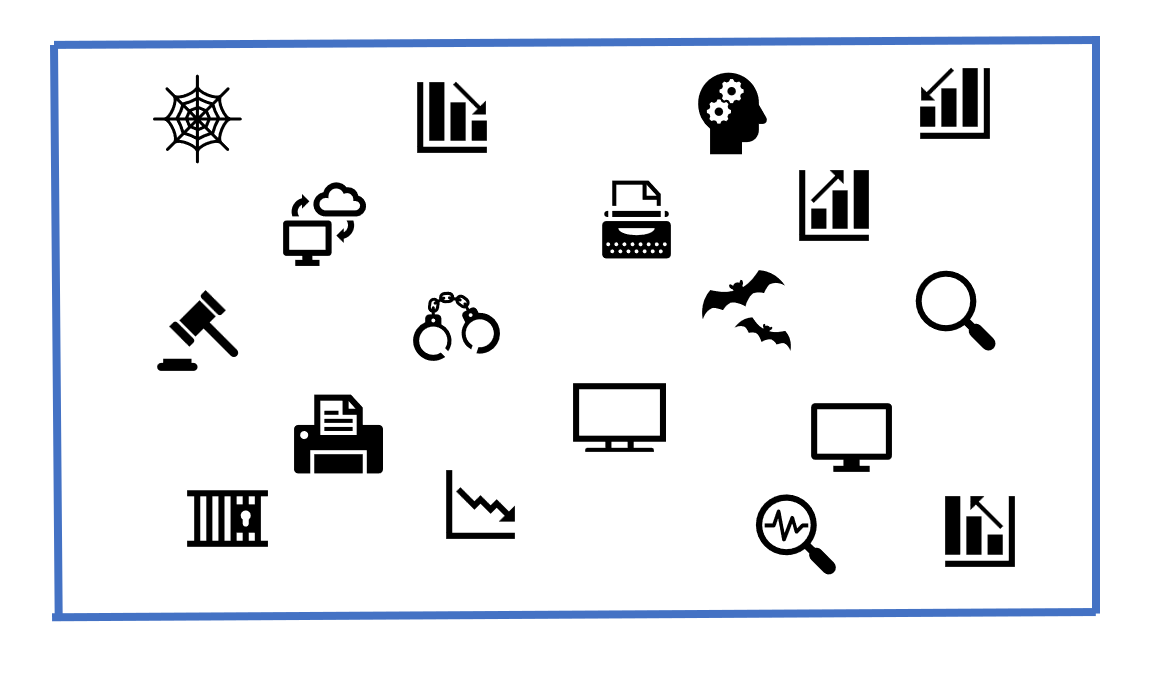
\includegraphics[scale=0.5]{template.jpg}
    \caption{模板图片}
\end{figure}

首先在园区全局内选定一处作为园区地图内的世界坐标系原点,考虑到整个地图的合理性,
选定的坐标系原点为校园中心位置。此处参考的地心坐标系统是WGS 84世界大地坐标系。
后续采集的点云数据均据此作为坐标系原点与位姿基准展开数据处理。

整个构建点云地图的流程框图如下所示:
\begin{figure}[ht]
    \centering
    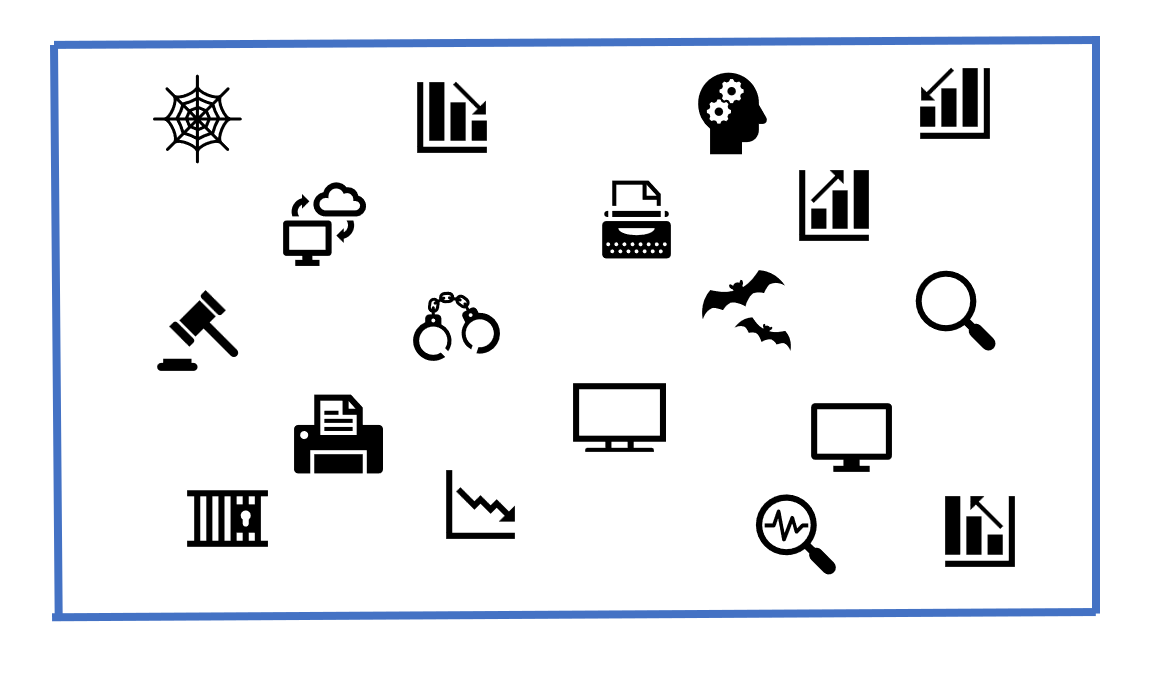
\includegraphics[scale=0.5]{template.jpg}
    \caption{模板图片}
\end{figure}

采集的软件系统为Robot Operating System(简称ROS系统)。采集地图的命令为:
sudo record -a;

\paragraph{地面提取}
地面提取的方式有多种,目前主流应用的是直接计算法、平面拟合法以及滤除法。其中直
接计算法是直接计算相邻两条激光线的俯仰角,俯仰角变化在一定范围内的可以被认为是
地面点;平面拟合法在底层导航一章中已经有叙述,主要是通过选取种子点拟合出相应平
面,并且通过迭代方法使得地面选取更加精准。再全局地图的构建过程中,由于不再是之
前简单将地面点去除,只需要迭代出地面后去除即可,关注点在于非地面点。此时我们对
于点云中地面点的质量有了更高的要求,是“宁缺毋滥”地筛选符合要求地地面点,人为增
加了点的筛选门槛。下面给出具体方法。
对采集得到的点云包进行分析,找到其中的velodyne\_points话题,对于包中所含有的
任意一帧点云进行分析,提取其中的非地面点部分与地面部分。提取地面部分点云的方法
如下所示:
对于激光雷达采到的任意一点,此点与激光雷达的位置关如下图所示:
\begin{figure}[ht]
    \centering
    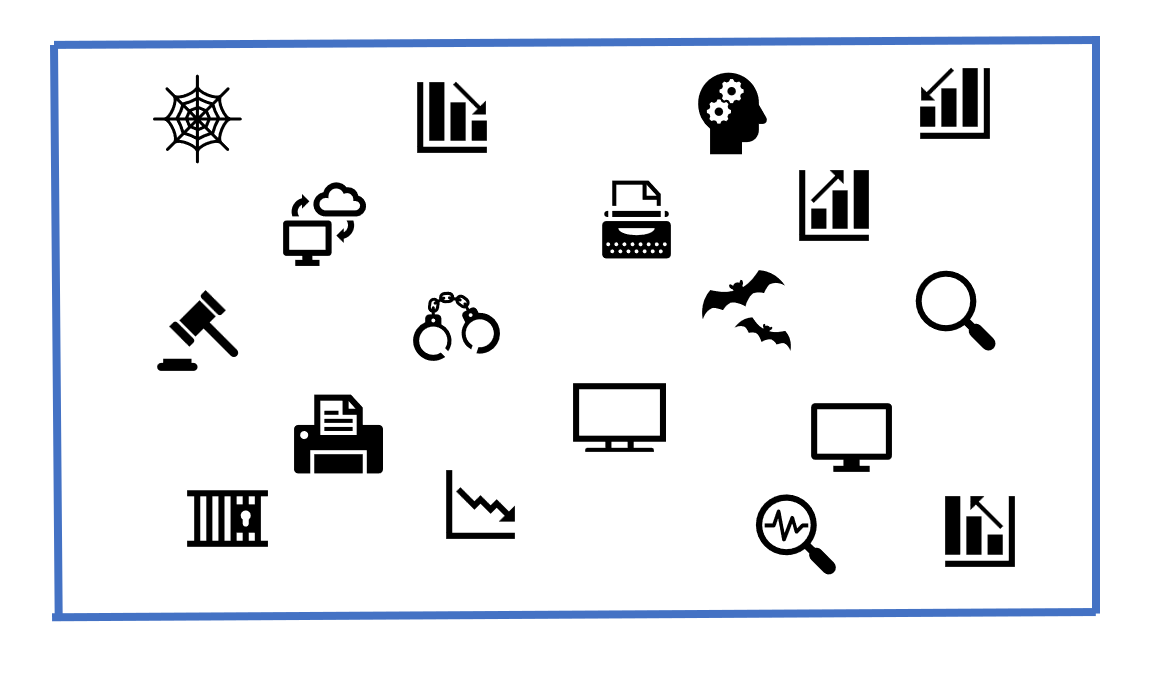
\includegraphics[scale=0.5]{template.jpg}
    \caption{模板图片}
\end{figure}

在激光雷达坐标系中,$\theta$ 表示点与水平xoy平面的夹角,x、y、z分别表示到坐标轴的距离
首先根据公式
\begin{equation}
    radius = \sqrt{x^2 + y^2}
\end{equation}
计算点的采集半径radius,再根据
\begin{equation}
    \theta = atan2(z ,radius) * 180 / \pi 
\end{equation}
计算得到点与水平面的夹角,atan2函数的象限划分与对应角度不同于atan函数,其原理为
\begin{equation}
\operatorname{atan} 2(y, x)=\left\{\begin{array}{ll}
    \arctan \left(\frac{y}{x}\right) & x>0 \\
    \arctan \left(\frac{y}{x}\right)+\pi & y \geq 0, x<0 \\
    \arctan \left(\frac{y}{x}\right)-\pi & y<0, x<0 \\
    +\frac{\pi}{2} & y>0, x=0 \\
    -\frac{\pi}{2} & y<0, x=0 \\
    \text { undefined } & y=0, x=0
    \end{array}\right.
\end{equation}

低于激光雷达坐标系xoy平面的点角度判定为-,而高于此平面的点角度判定则为+。
得到了某点的角度$\theta$,根据VLP-16激光雷达的角度分布,便可以得到某点所属于的
扫描线序号scanID,根据地面扫描点主要集中于最下面的三条扫描线的特点,只取角度为
-15°、-13°、-11°的三条扫描线上的点进行分析。
根据scanID将属于某条扫描线的点集合起来,检测点的粗糙值,粗糙值的计算公式为
\begin{equation}
    c_i=\frac{1}{|P|}\sum_{j\in P, j \ne i }||p_i-p_j|| 
\end{equation}
表达式的意思是首先取当前点同scanID的前后各十个点,$c_i$表示当前点的平滑度,P表示
当前点与其前后十点的集合,|P|值为邻点的数量,$p_i$、$p_j$分别表示当前点的向量与
其邻点的向量,对向量取2-范数。最终的平滑度表示为当前点与其周围——同一扫描线前后各10
点之间的距离均值。
并且在最后对下三线上的点完成分析之后,设置相应阈值,使得地面点合格率约为1/3左右。
最终,通过此方法取得的地面点在保证了点密度的情况下最大限度保证了地面点的质量。

\paragraph{基于RTK的地图合成}
每一帧地面点云地数据拿到之后,需要对地面点云根据位姿进行拼接,拼接点云地位姿来源于
数据采集过程中同时间戳录制的RTK位姿数据。
在前面fast\_gicp的叙述中也有提到两帧不同位姿的数据如何进行拼接,其实就是统一坐标系的
过程。与之前不同的是,之前的拼接没有一个全局的参考坐标系,是对车身位置实时位姿变换。
当在园区场景内选定了全局坐标系之后,若某一帧点云的位姿相对于全局位姿的变换为R、t,分
别表示点云帧相对于全局位姿所作的旋转与平移。
任意时刻,某点与当前坐标系的位置示意图如下所示。
\begin{figure}[ht]
    \centering
    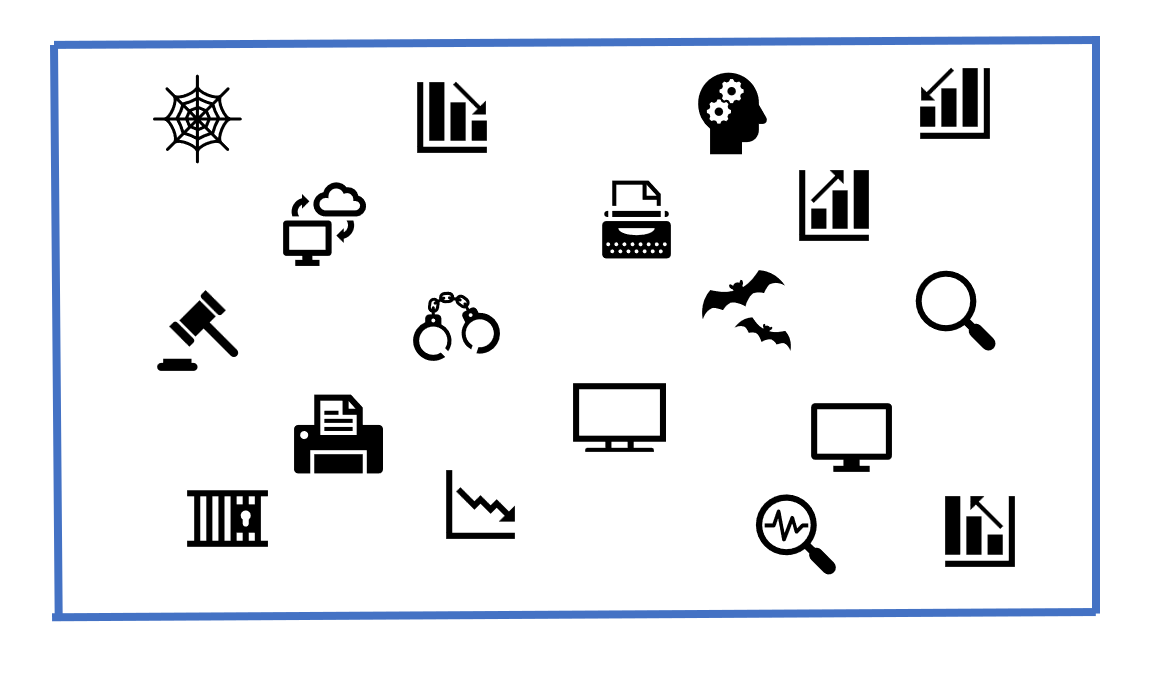
\includegraphics[scale=0.5]{template.jpg}
    \caption{模板图片}
\end{figure}
将当前点云中某点变换到全局坐标系下的变换为
\begin{equation}
    P'_1 = \symbf{R} * P_1 + \symbf{t}
\end{equation}


$P_1$表示点云的中某点的向量$[x,y,z]^T$,当前位姿,$P'_1$表示变换到全局坐标系下的位姿$[x',y',z']^T$。
该式还可以通过齐次坐标和变换矩阵的形式表现
\begin{equation}
    \begin{aligned}
    P'_2 = \symbf{T} * P_2 \\
    T=\begin{bmatrix}
        R& t\\
        0^T&1
      \end{bmatrix}
    \end{aligned}
\end{equation}
$P_2$表示点云的中某点的向量$[x,y,z,1]^T$,当前位姿,$P'_2$表示变换到全局坐标系下的位姿$[x',y',z',1]^T$。

此处可以直接调用pcl::transformPointCloud将一帧地面点云位姿变换到全局坐标系下,此过程仍然需要在一定帧数
拼接完成后进行降采样操作。操作原理与上一章类似。至此,地面点云的点云地图拼接完成,效果如下所示。
\begin{figure}[ht]
    \centering
    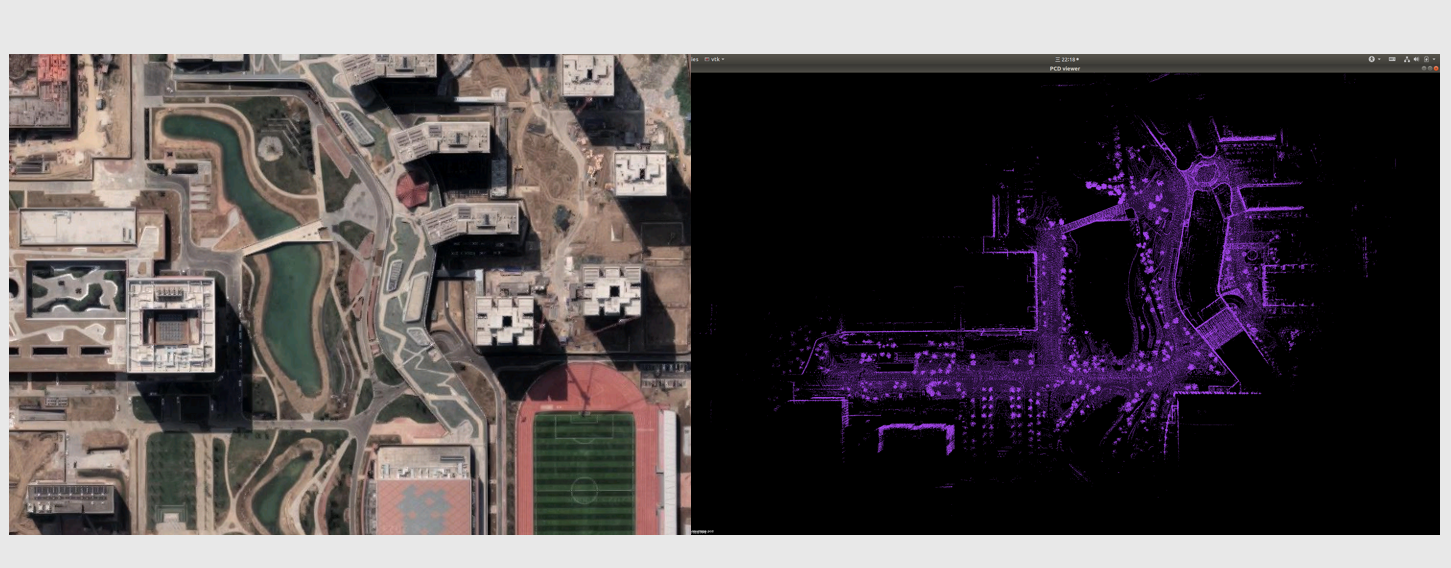
\includegraphics[scale=0.45]{globalPointsMap1.png}
    \caption{全局点云地图与原图片对比}
\end{figure}

\textcolor{red}{\underline{可以添加一部分用来讨论WSG84到RTK站心坐标系的转换}}

\subsubsection{栅格地图}
在得到了上述的地面点云地图roadMapAll之后,开始需要对这些可行使区域进行栅格化。在实际使用过程中,栅格化不必要对整个点云
地图进行,只需要对需要的可行驶区域部分,也就是上述得到的地面点云地图进行栅格化操作。
第一步获得此roadMapAll中点的极限值——所有点中最小的x值,y值,z值以及最大的x值,y值,z值。
依据此值对整个roadMapAll区域进行划分,按照0.5*0.5m的分辨率得到相应的栅格地图,每一个方格内所有点的平均高度为gridAverageHeight;


\paragraph{泛洪算法}
接下来使用著名的泛洪算法中的四邻域泛洪法,

\paragraph{腐蚀算法}
腐蚀算法主要目的是刻蚀掉孤悬于主区域之外的零星可行驶区域,此区域与其他可行驶区域的连接性不强,我们是不希望它作为后续路径规划的
节点网格的。





\subsection{基于距离地图的全局路径规划算法}
在选定的栅格地图基础上,进行全局的路径规划,规划时不考虑全局地图上的动态性,默认全局地
图上的可行驶区域在规划时刻均为静态可通行。一般来说,全局规划的算法有很多种,例如RRT、
RRT*、A*、Hybird A*、D*、Dijkstra等等。其中RRT簇适用于随机规划路径,但规划出的路径
不是最优的;A*簇算法适用于具备全局地图情况下的规划,并且规划出的路径是最优路径,其衍生
算法D*可以在地图有改变的情况下进行局部重规划;Dijkstra算法是一种BFS式的搜索算法,与A*类
算法相比,具有较高的搜索代价。由于我们提前说明不考虑全局地图上的动态性,故在全局搜索中
使用的是A*规划算法。

\subsubsection{A*算法}
原理简述:A星算法是一种常用于寻路问题的算法,可以在图形图像中找到从一个起点到一个目标点
的最短路径。一共如下3大步骤:
初始化起点和终点:首先将起点加入open列表,open列表存放所有待考虑的节点。同时初始化g值
和h值,其中g值是起点到当前节点的距离,h值是当前节点到终点的估计距离(如欧几里得距离)。

循环直到找到终点:在每次循环中,从open列表中选取f值最小的节点作为当前节点,并将其移入
closed列表中。如果当前节点为终点,则搜索完成。否则,将当前节点的邻居节点(即可以直接到
达的节点)加入open列表中,计算它们的g和h值。如果邻居节点已经在closed列表中,或者g值更
大,则不做处理。否则,更新g值,重新计算f值。

最终路径的生成:当终点被找到时,从终点开始按照每个节点的父节点反向寻找路径,直到回到起
点为止。这就是从起点到终点的最短路径。
A星算法的优点在于可以通过启发式函数对估计的距离进行优化,使得算法能够快速找到最短路径。同时,算法能够在不考虑地形的情况下进行路径规划,这使得它在游戏设计、机器人路径规划等领域得到了广泛应用。

A*算法的问题可以描述为
\begin{figure}[ht]
    \centering
    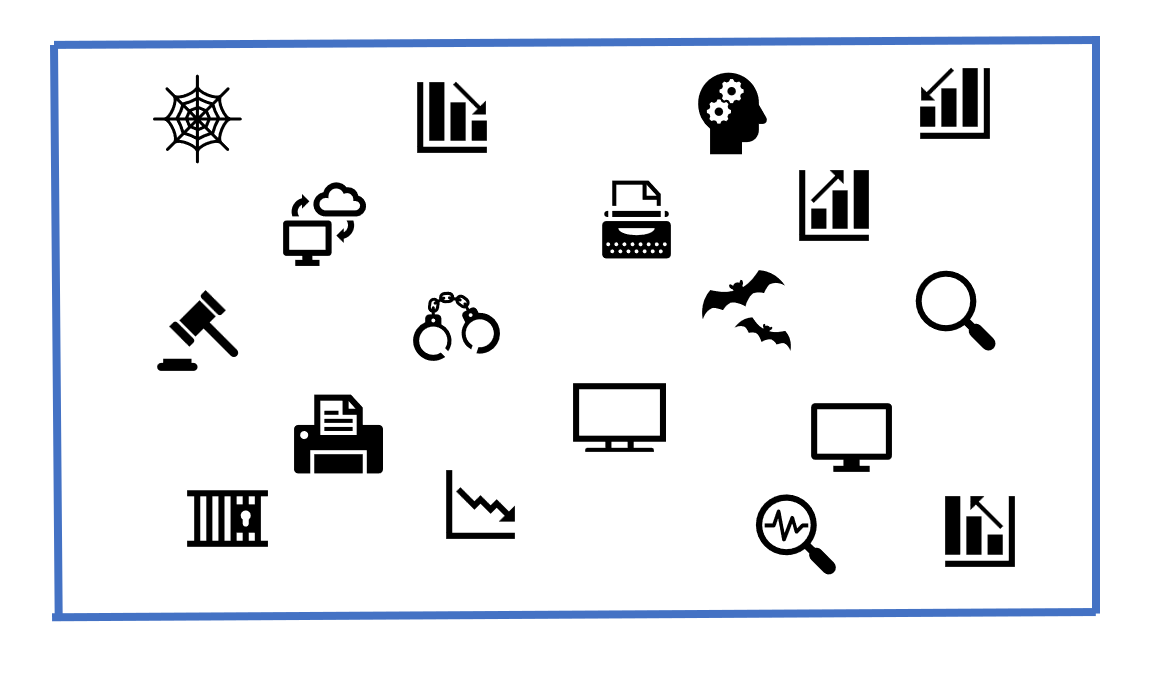
\includegraphics[scale=0.5]{template.jpg}
    \caption{模板图片}
\end{figure}

如何穿过避开障碍物并且在最小消耗的情况下到达终点位置。

在A*算法中最重要的是启发函数的设置,通常规律下,A*算法的启发函数可以描述为
\begin{equation}
    F = \alpha G +\beta  H
\end{equation}
其中,F表示总代价

G = 从起点 A 移动到指定方格的移动代价,沿着到达该方格而生成的路径。
H = 从指定的方格移动到终点 B 的估算成本。这个通常被称为试探法,因为
这是个猜测。直到我们找到了路径我们才会知道真正的距离,因为途中有障碍物
阻挡于当前网格节点与终点之间。
通过调节G与H的系数$\alpha$、 $\beta$ 可以对搜索的方式进行调整。例如当在距离地图中希望规划出的路径远离地图场景中
本就存在的障碍物时,便可以将H调整为到终点的估算成本与周围障碍物距离的加权和。




\section{基于局部点云的底层导航方法研究}

\subsection{基于Fast-GICP的局部点云}
导航系统的主要感知设备为Velodyne的VLP-16型号的激光雷达,雷达的主要参数为:
测量距离100m,360°水平视场角,\pm 15°的垂直视场、竖直分辨率2°、水平分辨率在
实验室移动机器人上10Hz下为0.2°。其中由于激光线束为16条,所以10Hz下扫描一圈的
单线采集点数为1800个激光点。这在园区场景下来说是十分稀疏的,导致在后面的避障
过程中无法有效对相应地点云进行信息处理,于是需要使用点云的技术拼接手段,将某个
范围内的点云进行融合,形成以车身为圆心的一定范围内的稠密局部点云。
此部分使用fast-gicp为算法主体,在其基础上,加入对点云帧的质心位置评估,使得
算法整体的实时性和可用性在实际场景中获得大幅度提升,免去了对很多边缘离群点的
计算量。


不同于全局地图中使用RTK获取移动机器人位姿,在底层导航的设计中,兼容了室内场景的应用模
式,使用Fast-GICP可以在室内进行应用。



\subsubsection{车身当前位置范围内点云帧选取}
为了得到当前时刻车身周围的稠密局部点云,需要保存车身圆周范围一定数量的点云帧,评
价某个时刻采集到的点云数据$\symbf{P}_t$与当前车身位置的距离,需要获取$\symbf{P}_t$
的质心,点云质心指的是点云的质量中心,通常被认为是点云的质量集中于此点的假想点。
质心的计算公式为:
\begin{equation}
    \begin{cases}
       \overline{x} = \frac{\sum\limits_{i=1}^{N}x_i}{N}\\
       \overline{y} = \frac{\sum\limits_{i=1}^{N}y_i}{N}\\
       \overline{z} = \frac{\sum\limits_{i=1}^{N}z_i}{N}\\
    \end{cases}
\end{equation}
其中$\overline{x}$、$\overline{y}$、$\overline{z}$分别表示此帧点云质心的坐标数
值。同时为了避免边缘噪点对于质心的计算影响,同时我们关注的点云也只限于车身范围内
的5m半径内,所以通常会将点云基于其采样中心的半径10m计算其质心,这样既省去了计算量,
由去除了采样帧远方边缘噪点的影响。事实上,在PCL库的内部已经集成了的相应的求取点云
质心的函数pcl::compute3DCentroid,只需要将相应的库加入文件中便可以调用。
选取车身当前范围的一定数量的关键帧方式如下,首先初始化,根据时间顺序,选取一定数量
的点云帧,完成初始化之后,基于位置信息的二维距离选取下一帧,并在移动的过程中,逐步
替换掉最早的点云帧,保证点云池内存在的点云帧数量保持为定值,点云帧的选取示意图如下:
\begin{figure}[ht]
    \centering
    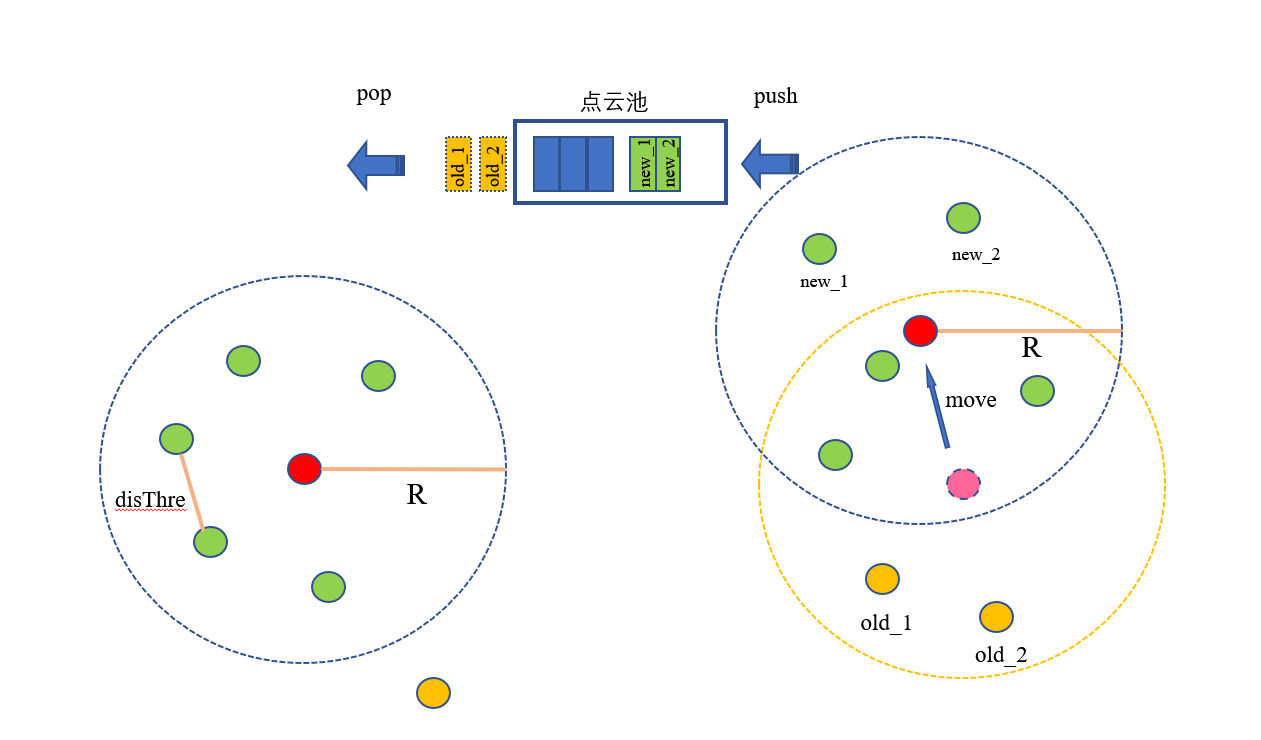
\includegraphics[scale=0.5]{pcselect.png}
    \caption{临近点云帧的选取}
\end{figure}
图中红色点表示当前车身所处位置,绿色、橙色表示车身范围内与外的邻近点云质心所处位置。
点云池内部的点的数量除了初始化时,始终保持数量不变,并且绿色点之间的距离有最小阈值
disThre限制。

\subsubsection{Fast-GICP点云拼接}
点云池内拥有一定数量的点云帧之后,对点云池内的点云进行拼接操作。
点云池内的点云与原采集到的点云保持对应关系,为保证ICP算法的精准度,将原始帧输入fast\_gicp
处理模块,由此得到相应帧之间的位姿关系,并且位姿关系对上述帧进行拼接。

\paragraph{Fast-GICP配准算法}
Fast Global Iterative Closest Point (Fast-GICP) 是一种用于点云配准的算法,是 Global 
Iterative Closest Point (GICP) 的一种改进。它通过使用局部高斯表达来计算点云间的相似性,
并通过加速矩阵求逆和构建雅可比矩阵的方式提高了配准的速度和精度。
Fast-GICP 的原理基本上是在 GICP 的基础上进行的改进。在 GICP 中,点云的对应关系是通过点
之间的欧氏距离计算的,而 Fast-GICP 则采用了点云之间的局部高斯表达,这有助于解决欧氏距离
在存在噪声或离群点时产生的误差问题。
Fast-GICP 还使用了一些技巧来加速矩阵求逆和构建雅可比矩阵,例如采用 SVD 分解来避免矩阵求
逆的计算和采用块状矩阵来优化雅可比矩阵的构建。这些技巧有助于提高配准的速度和精度,并使 
Fast-GICP 成为一个非常有效的点云配准算法。
其算法步骤为:

\begin{enumerate}
\item 定义目标点云和源点云 $Target$ 和 $Source$,其中 $Target$ 是固定点云,$Source$ 是需要变换以匹配 $P$ 的点云。

\item 初始化初始变换矩阵 $T_0$,通常情况下可以将变换矩阵初始化为单位矩阵,以便于进行迭代,即$T_0$ = $I$。

\item 对于每次迭代:

a. 通过应用当前变换矩阵 $T$,将 $Source$ 变换到当前位置。

b. 计算 $Target$ 和 $Source$ 之间的最近点对,并计算最近点对之间的距离,距离计算公式为
\begin{equation}
    d(p_i, q_j) = ||p_i - Rq_j - t||
\end{equation}
其中$p_i$表示点云Target中的第$i$个点,$q_j$表示点云$Source$中的与$q_i$最近的点,$R$,$t$分别表示
当前变换矩阵$T$的分解处的旋转向量与平移向量。

c.根据最近点对计算点的权重
\begin{equation}
    \omega (p_i, q_j) = exp(-\frac{d(p_i, q_j)^2}{2\sigma ^2})
\end{equation}
其中$\sigma$是一个常数,用于控制高斯函数的宽度。

d.计算均值向量
\begin{equation}
    \mu_{Target} = \frac{1}{N}\sum_{i = 1}^{N}p_i,  \mu_{Source} = \frac{1}{N}\sum_{j = 1}^{N}q_j
\end{equation}
其中$N$表示点云中的点数。

e.计算协方差矩阵
\begin{equation}
    H=\sum_{i=1}^{N} w\left(p_i, q_j\right)\left[\begin{array}{ll}
        q_j & 1
        \end{array}\right]^{T}\left[\begin{array}{c}
        p_i-\mu_P \\
        1
        \end{array}\right]\left[\begin{array}{c}
        p_i-\mu_P \\
        1
        \end{array}\right]^{T}\left[\begin{array}{ll}
        q_j & 1
        \end{array}\right]
\end{equation}

f.SVD分解$H$矩阵
\begin{equation}
    \begin{aligned}
    H = U \sum V^T \\
    R = VU^T \\
    t = \mu _P - R\mu _Q
    \end{aligned}
\end{equation}  
其中,$U$ 和 $V$ 是 $H$ 的左奇异向量和右奇异向量,$\Sigma$ 是 $H$ 的奇异值矩阵。

d. 更新变换矩阵 $T=T_{corr}T$,并且更新点云$Target$中的点。
\begin{equation}
    p_i \leftarrow Rp_i + t
\end{equation}

    \item 如果达到停止条件,则返回最终变换矩阵 $T$,否则返回步骤 3。

\end{enumerate}

\paragraph{局部点云生成}
Fast-GICP作为算法主体生成局部点云,其流程图如下:
\begin{figure}[ht]
    \centering
    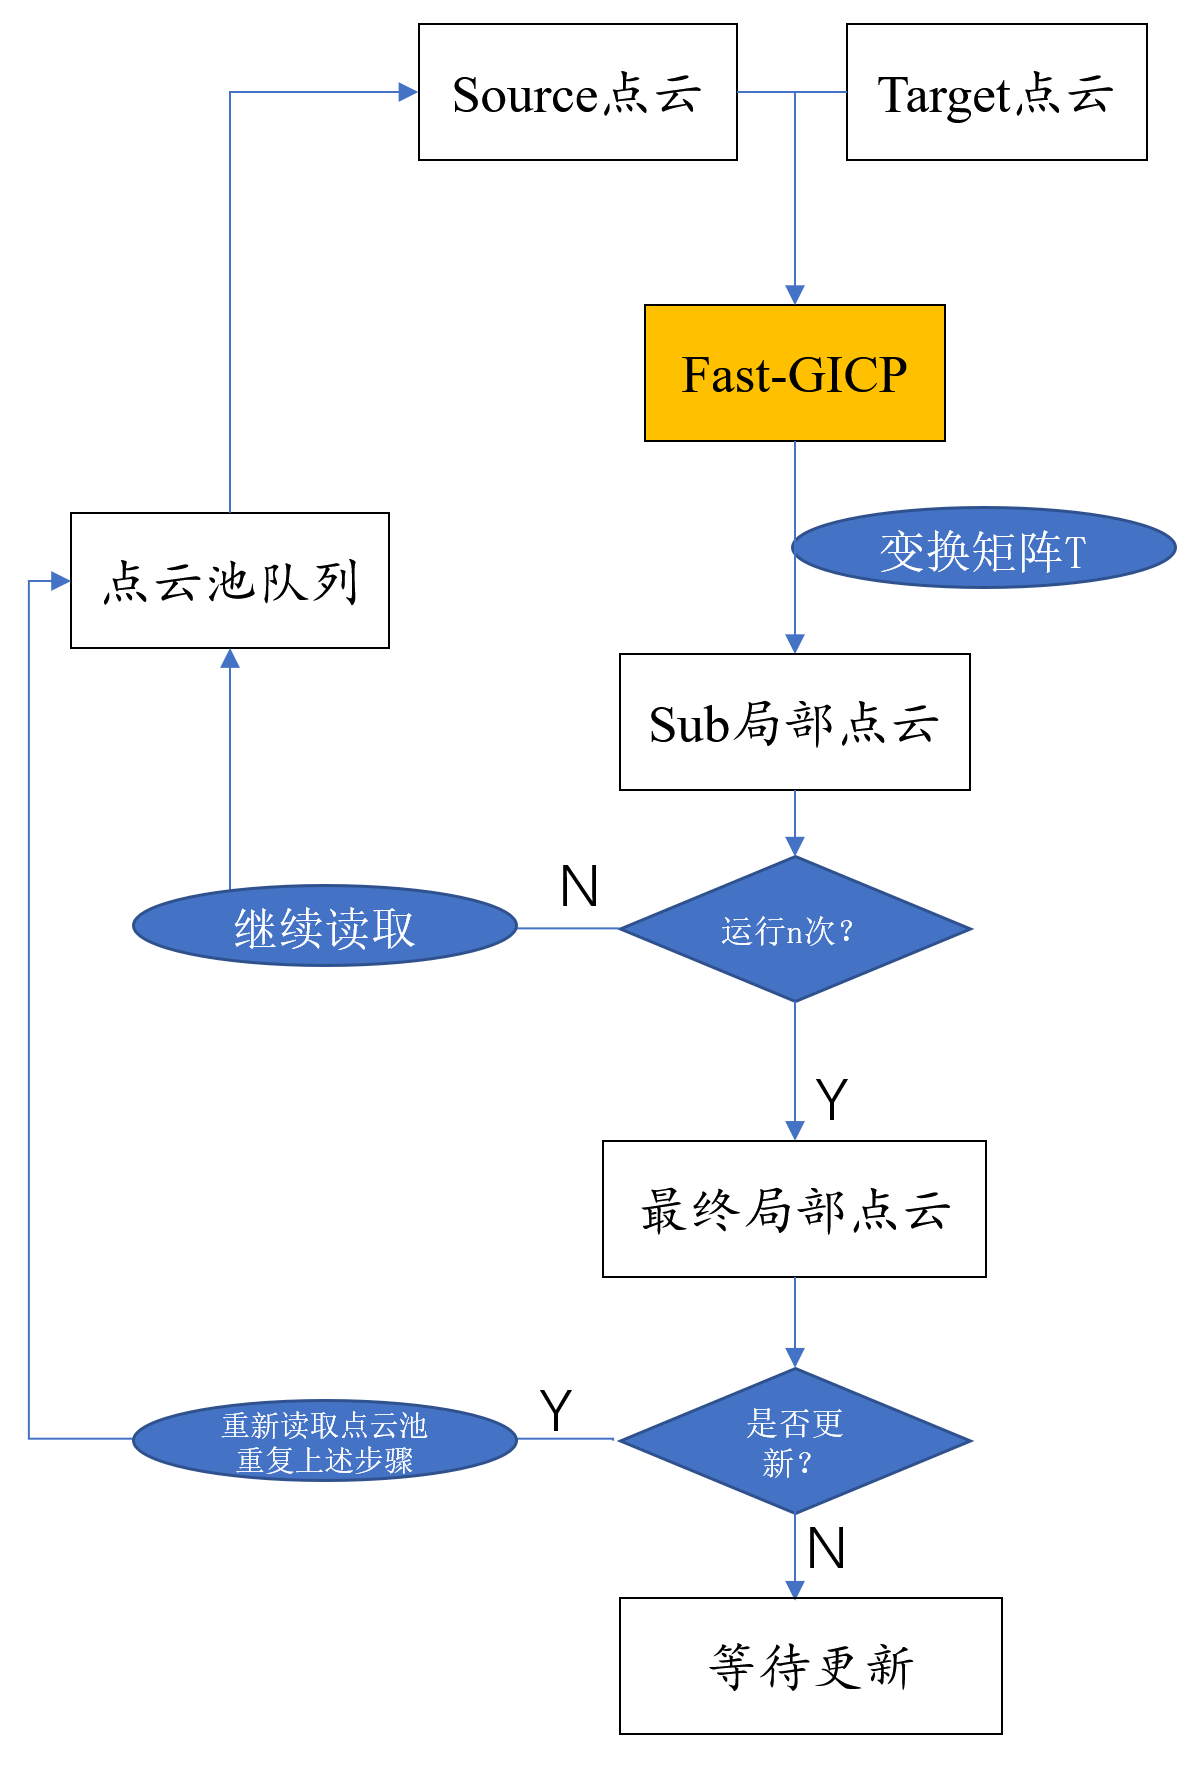
\includegraphics[scale=0.45]{localPointCloud1.png}
    \caption{局部点云生成过程流程图}
\end{figure}
初始化时,$Source$点云是从点云池队列中进行读取,$Target$点云则是采集车身当前时刻的
点云,通过Fast-GICP算法配准后,合成sub局部点云地图。当参与构建局部点云的点云帧到达阈值
$n$($n$为点云池内点云帧总数),初始化完成,第一个局部点云构建完成。
当完成初始化之后,点云池队列中的点云数量更新达到阈值后,即当点云池内部点云帧数量更新第
$\frac{3n}{4}$帧时,说明此时小车距离上次生成局部地图的位置已经足够远,在运行则要离开当前局部
点云的范围,此时更新局部点。

经过此步骤,拼接得到的局部点云效果图如下:
\begin{figure}[ht]
    \centering
    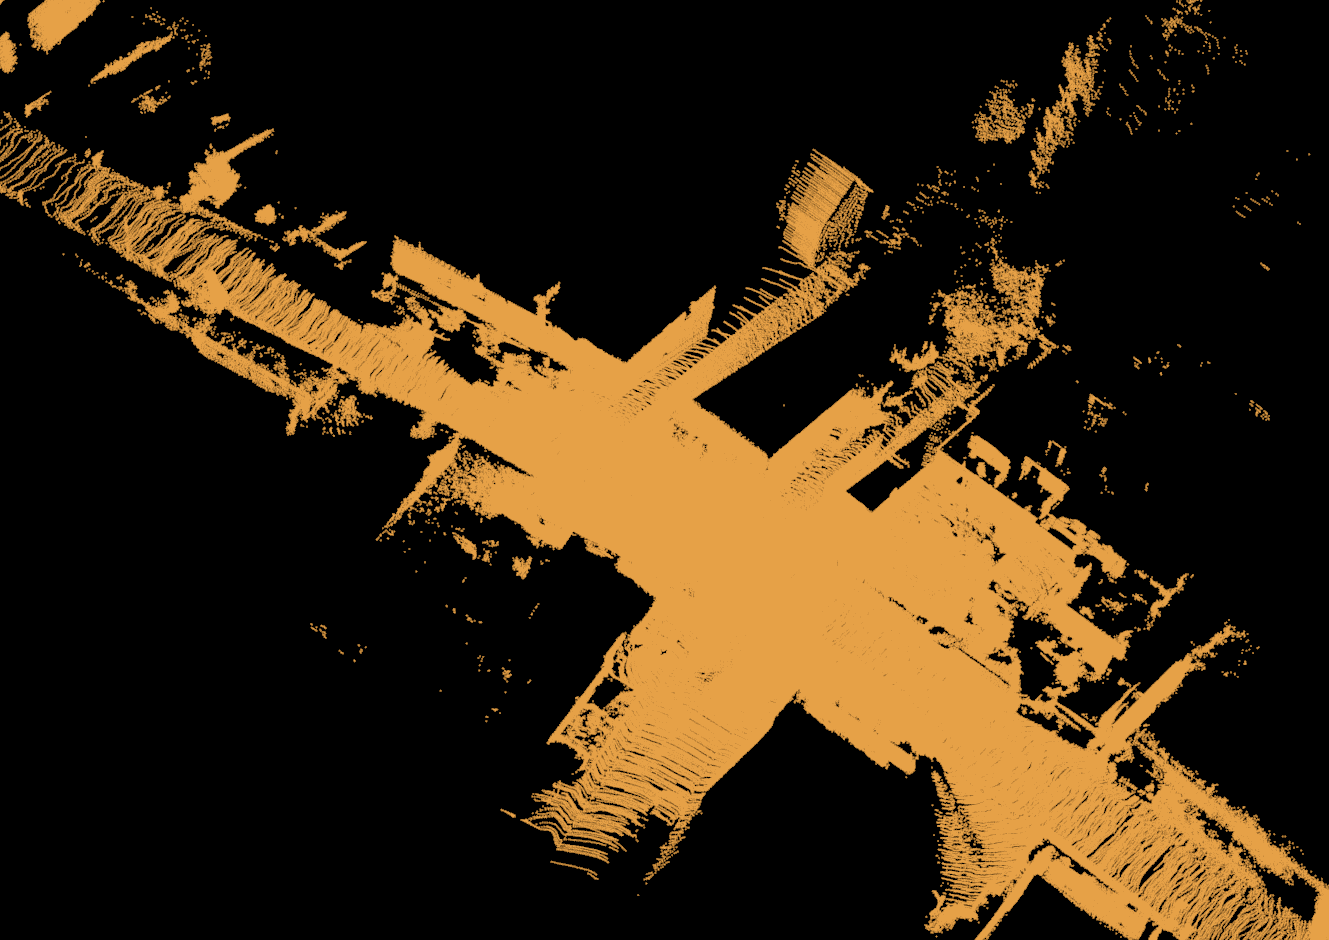
\includegraphics[scale=0.25]{localMAP.png}
    \caption{经过拼接的初始局部点云}
\end{figure}



\subsubsection{稠密点云降采样}
激光点云经过拼接后,同一物体处的扫描点迅速增加,影响后续算法的实时性。
对得到的局部稠密点云进行适当的降采样,可以使得局部点云信息更加清晰,条理分明。
得到的局部点云地图是经过点云配准算法的处理,其中多了冗余信息与噪点,直接处理
计算量资源消耗巨大,因为降采样是必要的操作。

降采样的方法有多种,例如体素网格下采样、均匀下采样、几何曲率下采样、随机下采
样等。这里选择的是体素网格下采样法。
体素的概念就是将空间划分成一个个立体的方格,每一个方格就称为一个体素网格,降采样
的思路是检查每个体素中是否有点存在,若哟,则用一个点代替体素内的点集,此处使用体素
网格中心点坐标作为采样点。体素网格降采样的优点是可以通过控制体素网格的分辨率控制
采样点之间的距离。

经过降采样后得到如下的降采样点云,对降采样算法的分辨率分别使用resolution = 0.25
、0.5、0.75,效果图分别如图(a)、(b)、(c)所示。
\begin{figure}[ht]
    \centering
    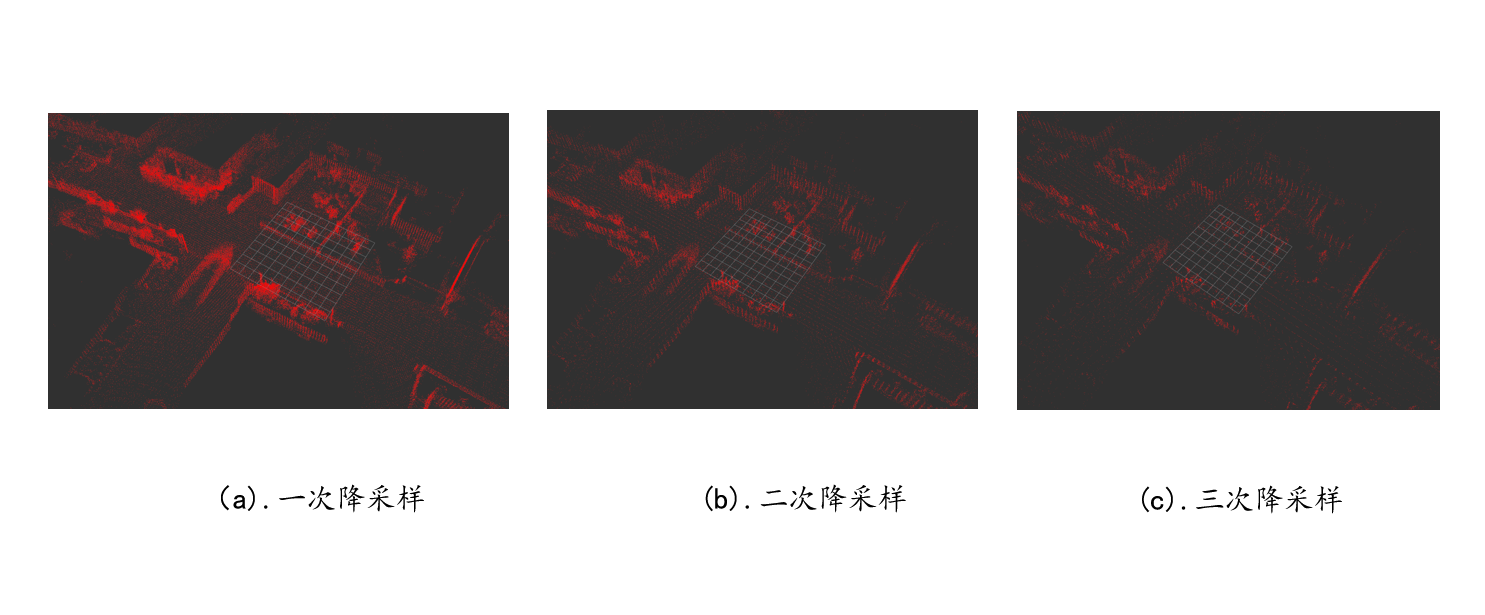
\includegraphics[scale=0.45]{downSample.png}
    \caption{降采样结果效果图}
\end{figure}


此步骤完成后,便可以得到以车身目前在环境中所处位置为基准的局部点云,根据此
可以开展点云的后续处理工作。



\subsection{局部点云的分割与聚类}
对当前的局部点云进行有效的分割处理并聚类,是接下来进行避障以及路径规划的基础,
点云的分割聚类主要是为了让底层导航系统在避障过程中识别障碍物,并且对动态障碍
物信息做出实时的反馈与动作。具体的分割与聚类工作如下。

基于Bogoslavskyi在文章Fast range image-based segmentation of sparse 3D laser
 scans for online operation" 2016 IEEE/RSJ International Conference on 
 Intelligent Robots and Systems (IROS).提出的点云聚类方法,在一些细节处理上
 进行了创新,并将创新后改进的程序用于了底层导航系统设计。

\subsubsection{扫描线补偿}
激光雷达的工作原理就是通过传感器发射激光光束并通过激光光束的返回时间差来实现对
周围环境的感知,返回的形式最终以激光点类型记录在相应的文件中。如果传感器发射的
激光雷达线束打在了反射率较低的物体上,会形成相应的点的缺失,例如车窗玻璃或者目前
随处可见的玻璃落地窗等,都容易造成对当前环境的误判。这就造成了分析上的困扰。可以
对得到的某一帧点云进行补缺,补缺的原理是通过线性插值的方式对确实的点进行补偿,方
法如下。
首先对无效点进行初步聚类,聚类得到的某一区域的无效点数量在阈值范围内,并且在阈
值范围内的无效点周边的障碍物点距离不超过1.5m,可以认为此处为确实的障碍物点,通过
线性插值的方式,对障碍物点内部包围的无效点进行补偿,补偿前的效果图和补偿后的效果图
如下图所示。
\begin{figure}[ht]
    \centering
    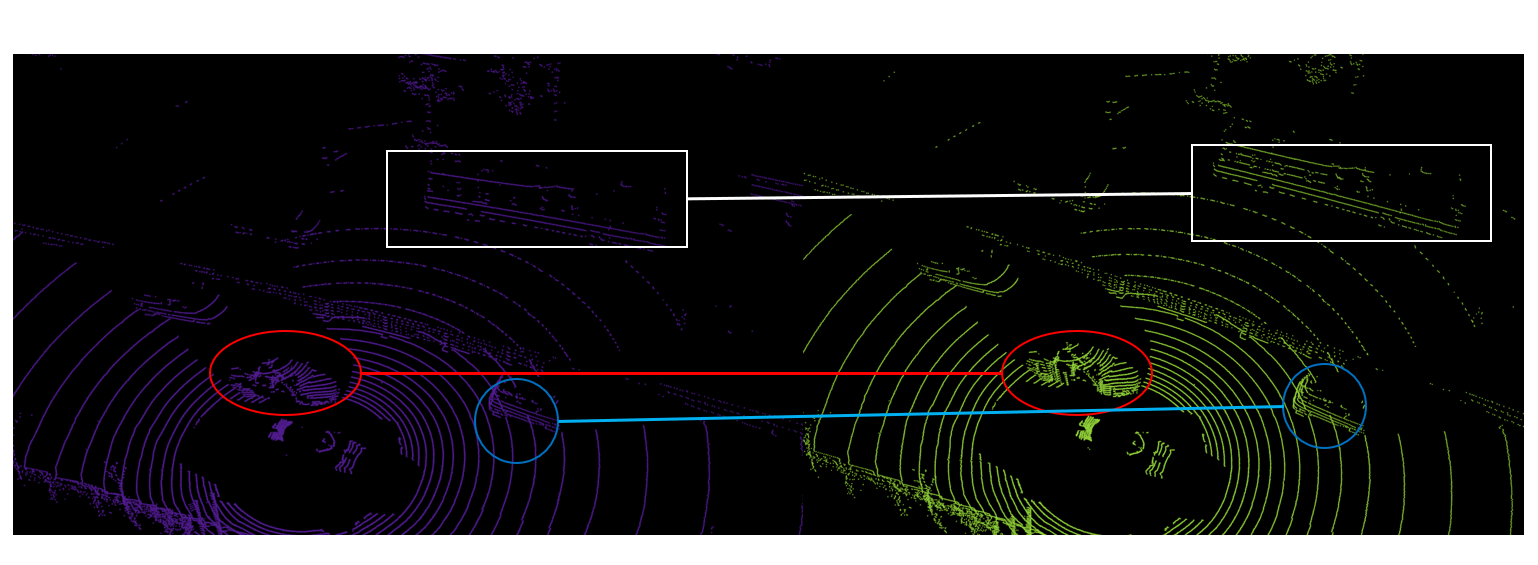
\includegraphics[scale=0.42]{scanline.png}
    \caption{扫描线补偿前后对比}
\end{figure}

\subsubsection{地形分析}
得到的局部点云是包含有静态物体、动态物体以及地面的综合帧,在处理数据的过程中,
地面点通常来说是一个不许要过多考虑的因素,但是需要得到相应的地面点云,作为局部规划中的
可行驶区域,并且得到地面点云之后才可以知道其他点相对于地面点的关系,得出此点是否是障碍物
的结论。在LeGO\-LOAM中,点云中的地面点是经过实时分割的,分离出地面点与非地面点之后
只保留非地面点部分进行数据处理。这样不仅可以降低计算量,也可以把去除地面点上一些干扰
因素。去除地面点的方法有很多,第一步,首先考虑如何找到一帧点云的地面点。实验室的移动
智能机器人上采用的是地面拟合法对点云中的地面点进行平面拟合。现实中激光雷达采集到的
地面点通常不是一个完美的平面,那么采取单一的平面模型来拟合点云中的地面时不显示且具有
相当大的噪点误差的。要完成相应的地面分割就需要对坡度进行一定的拟合,而不能够把坡度
视为非地面点。通过将地面空间沿着$\symbf{x}$方向,分成若干个子平面,对每一个分割出的
子平面进行地面平面拟合算法(GPF)进行拟合。
GPF的拟合算法如下所示:
\begin{algorithm}[ht]
    \SetAlgoLined
    \KwData{this text}
    \KwResult{how to write algorithm with \LaTeX2e }
  
    initialization\;
    \While{not at end of this document}{
      read current\;
      \eIf{understand}{
        go to next section\;
        current section becomes this one\;
      }{
        go back to the beginning of current section\;
      }
    }
    \caption{算法示例1}
    \label{algo:algorithm2}
  \end{algorithm}
对于任意一帧点云$P$,最终的分割聚类的目的是将其分成$P_g$以及$P_ng$,即地面点和非
地面点。算法在应用过程中,有四个十分重要的参数分别是$N_iter$、$N_lpr$、$TH_seed$、
$TH_dist$,它们的意义是分别代表进行拟合迭代的次数、用于进行地面平面拟合的最低点代表
(lowest point representative)的数量、选取种子点的阈值(点云中某点的高度低于最低点
代表的高度和此阈值的和时,将此点加入种子点序列)、用于判断当前点云某点与拟合出的平面
的正交投影距离的阈值(低于此阈值,则将此点加入$P_ng$)。

对输入得到的点云按照点云中每个点的z轴竖直进行排列,取$N_lpr$个最低点代表,并求得这些
代表的均值lpr\_height。如果某点的$p_z$
\begin{equation}
    p_z  < lpr\_height + TH\_seed 
\end{equation}
那么便将此点加入种子点序列。
确定平面模型时候,选择最基本的线性模型用于估计平面,线性模型
\begin{equation}
    \begin{aligned}
    a x+b y+c z+d=0\\
    \symbf{n}^{T} \mathbf{x}=-d 
    \end{aligned}   
\end{equation}
这其实是一个公式,下式是对公式的向量化,其中$\symbf{n}$ = $[a,b,c]^T$,$\symbf{x}$ = $[x,y,z]^T$
,通过初始点集的协方差矩阵即可求得$\symbf{n}$,从而确定出一个平面。
采用种子点集为初始点集,通过公式
\begin{equation}
    C=\sum_{i=1:|S|}\left(s_{i}-\hat{s}\right)\left(s_{i}-\hat{s}\right)^{T}
\end{equation}
其中$\overline{s}$表示所有点的均值,其中协方差矩阵的三个向量可以通过奇异值分解(SVD)的方式
求得,最终获得整个平面的法向量$\symbf{n}$。
上述得到这个初始的平面模型以后,会计算点云中每一个点到该平面的正交投影的距离,并且将这个距离与
设定的阈值$TH_dist$比较,当高度差小于此阈值,认为该点属于地面,当高度差大于此阈值,则为非地面点。
经过分类以后的所有地面点被当作下一次迭代的种子点集,迭代优化,在实际操作中选择的迭代次数为3次,
既保证迭代出的平面拟合性,也可以保护计算资源。
最终将拟合得到的去除地面点后的点云图以及地面点云分别如图所示:
\begin{figure}[ht]
    \centering
    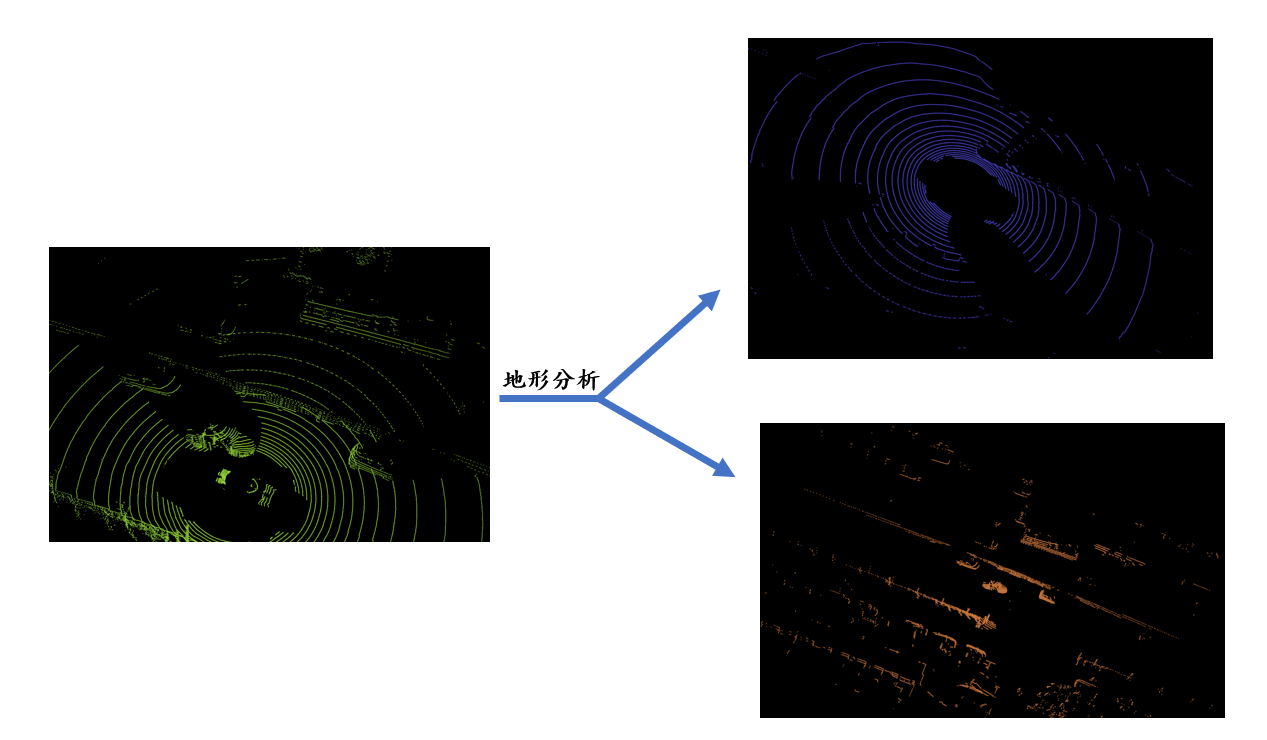
\includegraphics[scale=0.45]{terrainAnalysis.png}
    \caption{地形分析结果效果图}
\end{figure}

得到了地面之后,根据拟合得到的地面对地面上的点与地面之间的高度进行分析,取其相对高度高于15cm的作为
Obastacle,即表示obstacle为障碍物点云,障碍物点云不可以直接通行,需要在避障模块中特殊考虑。高度在
拟合地面与障碍物最低阈值之间的,视作斜坡,主要在局部导航的路径选择中作为权重之一,旨在选择出相同条件
下,代价最低的局部路径。

% \subsubsection{深度图生成}
% 深度图指的是将点云的数据转化成平面型数据进行下一步的邻域搜索,在存储过程中可以存入相应点的信息,例
% 如点的距离与强度信息,在得到点的位置之后,某一点的其他位置都会在深度图中体现出来,不需要进行对点距离
% 分析,搜索其邻点。
% 此处使用哈希表来存储点的位置信息与其强度信息(或者称为距离信息),其中的键值用以存储当前点的位置,例
% 如对于一帧高为hight,宽为wid的cv:Mat来说,某一个点的像素位置为(row,col)对应的哈希表键值index存储为
% \begin{equation}
%     index = row*wid + col 
% \end{equation}
% 最终构建出的深度图如图所示:


\subsubsection{BFS聚类方法}
地形分析之后得到的地面点云与非地面点云,地面点云理所当然作为可行驶区域,不用做更加特殊化的处理。
而对于非地面点云,则需要进行进一步的分割。
首先对于非地面点云的聚类,进行四邻域搜索之后,设定阈值,将一定阈值内的点判断成为相同点簇,过程中
可能会出现同一物体由于扫描角度等问题被分割成为两个点簇,故需要对两个点簇内的点进行角度判断,以确定
两簇点云是否属于同一物体。
如图,当两簇点云进行比对时,若任意两个点之间的角度$\theta$ > $\lambda$ ,则表示两点属于同一物体,
$\lambda$表示判断阈值。
\begin{figure}[ht]
    \centering
    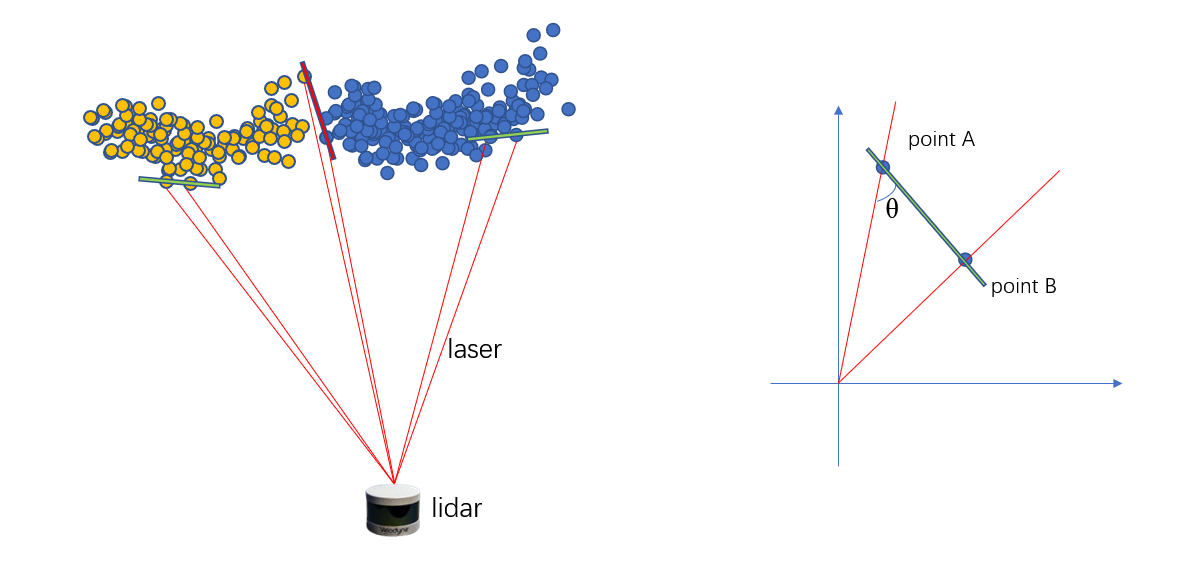
\includegraphics[scale=0.45]{angleThre.png}
    \caption{点簇融合与分割角度比较}
\end{figure}

\subsection{底层局部规划器设计}
本章上述几个模块已经对相应的环境信息进行了处理,并且可以拿到处理过后的环境点云信息。本节的具体内容是
根据拿到的环境信息进行局部规划器的设计,规划器的设计参考了CMU团队的思路理念,融合实验室移动机器人的
阿克曼底盘模型,构建出了基于阿克曼模型的底层导航规划器。底层规划器的主要任务是处理相应的环境信息,订阅
机器人在当前环境中的位置,将高层导航下发的次级目标点解算成为当前移动机器人所需要行走的方向与相应的速
度。


\subsubsection{阿克曼底盘的轮式里程计模型}
使用阿克曼底盘进行规划时,必须对阿克曼底盘的里程计模型进行了解,以进行正确的控制空间点采样。
阿克曼的轮式里程计(以下简称轮式里程计)是根据车辆的运动学模型,将车辆的轨迹模型进行累计,
得到车辆的运行里程的一种技术手段(以前此术语指的是一种仪器,现在多指一类技术方法,例如视觉
里程计)。
如图所示,现在有一个阿克曼结构的底盘模型示意图,如图。
\begin{figure}[ht]
    \centering
    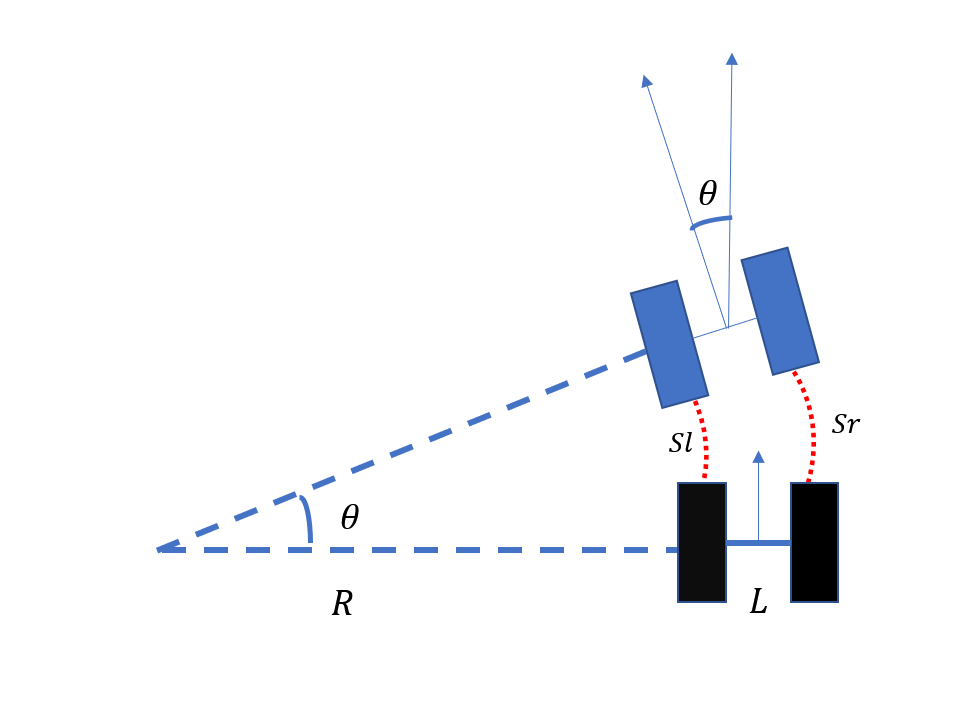
\includegraphics[scale=0.5]{ackerman.png}
    \caption{阿克曼结构示意图}
\end{figure}

阿克曼结构左右轮在转向时所走的距离不同:$\symbf{R}$为转动半径,$\theta$ 为转动角度,$\symbf{L}$为阿克曼轴距。
其中:
\begin{equation}
    \begin{cases}
        \symbf{s}_{\symbf{l}} = \theta \symbf{R}\\
        \symbf{s}_{\symbf{r}} = \theta (\symbf{R} + \symbf{L})        
    \end{cases}
\end{equation}

将两边的等式同时除以时间,进一步可以得到:
\begin{equation}
    \begin{cases}
        \symbf{v}_{\symbf{l}} = \omega  \symbf{R}\\
        \symbf{v}_{\symbf{r}} = \omega (\symbf{R} + \symbf{L})        
    \end{cases}
\end{equation}
最后再将两式联立可得:
\begin{equation}
    \omega = ( \symbf{v}_{\symbf{r}}- \symbf{v}_{\symbf{l}}) / L
\end{equation}
证明阿克曼结构的角速度是相同的,更进一步,可以把阿克曼模型等效成为自行车结构,
对于移动机器人向前运动的情况,$\symbf{x}$ 、4$\symbf{y}$ 和$\theta$ 三个维度上
的速度分别为:
\begin{equation}
    \begin{cases}
        \dot{x} = \symbf{v}\cos \theta \\
        \dot{y} = \symbf{v}\sin \theta \\
        \dot{\theta } = \frac{\symbf{v}\tan \theta}{\symbf{L}}
    \end{cases}
\end{equation}
为了在计算机中表示和便于计算,我们将基于阿克曼底盘的运动学模型离散化为空间中
的一系列点。这样,从初始时刻的初始位置出发,可以由前一时刻t的位置递归推导出
t+1时刻的位置和旋转角度。 该方程表示为:
\begin{equation}
    \begin{cases}
       x_{t+1} = x_{t} + v_{t}\cos(\theta _{t})d_{t}\\
       y_{t+1} = y_{t} + v_{t}\sin(\theta _{t})d_{t}\\
       \theta_{t+1} = \theta_{t} + \omega_{t}d_{t}
    \end{cases}
\end{equation}

相应地,根据该离散公式可以得到对应的适用于阿克曼运动学约束的离散路径集。

\subsubsection{向前模拟三次样条生成离散路径组}

在有了上面的阿克曼模型的里程计空间方程之后,以车辆的后轮中心为base\_link,以
base\_link为起点,按照阿克曼里程计模型,向前模拟三次,生成相应的离散路径组。
离散路径组的示意图如图3.5所示,路径的转向范围是-22.5°~22.5°,完美贴合煜禾森FR-07
的车身转向范围。
\begin{figure}[ht]
    \centering
    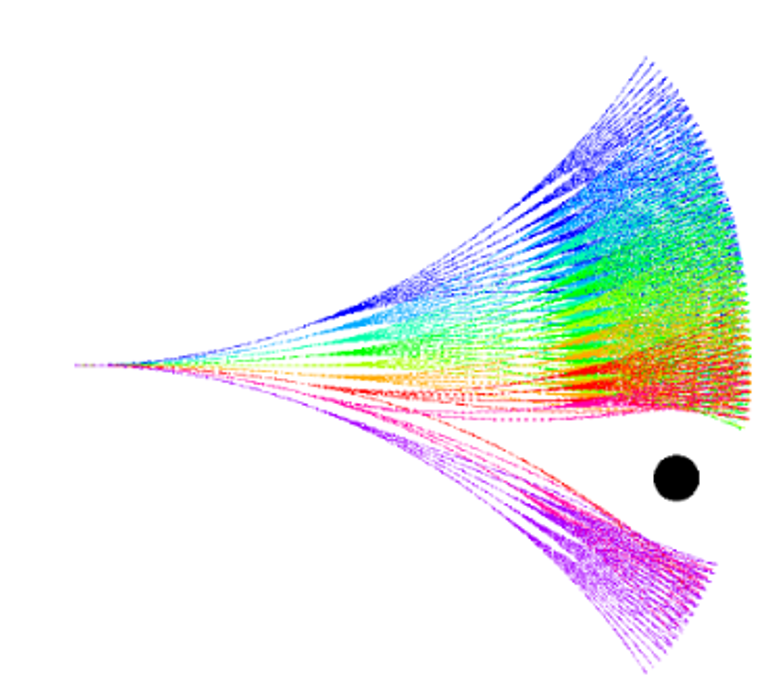
\includegraphics[scale=0.5]{paths.png}
    \caption{离线路径组示意图}
\end{figure}
第一次将45°转向范围分为9个等分,每5°生成一条路径,然后按照此方式,在生成的9条路经的基础上二次模拟,直到三次模拟全部完成,共生成9*9*9条路径,一共分为9个group,每个group种存有9*9条路径。

其中,图中黑色圆点表示有障碍物占据时,影响到的路径组数量。此处考虑了车身的本身具有的
轮廓,路径的任何位置占据导致车身轮廓与障碍物点的碰撞,都会被视为影响路径。下文将详细叙述此部分。

将此路径组以一定的频率发送给底盘的后轮中心,并且需要注意的是,实际使用时候要将激光雷达扫射在移动
机器人身上的部分,将这一部分的影响去除,因为车辆本身并不会撞到小车自身。
在得到某一个目标点之后,局部规划期开始工作。

\subsubsection{依据点云信息判断路径上障碍物的方法}

车身位置与路径组的关系如下图所示。路径组由车身后轮中心位置延伸出来,并且对路径组原点以棋盘中心,
构建体素网格,体素网格与路径组内的点具有离线构建的对应关系。对应关系如下图所示:
\begin{figure}[ht]
    \centering
    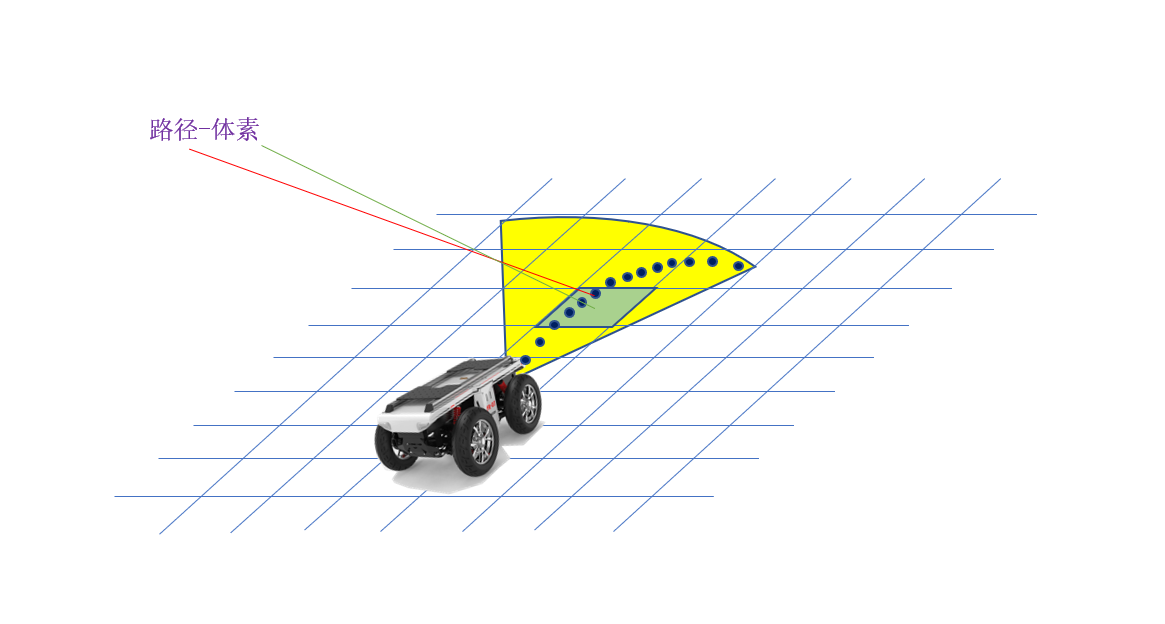
\includegraphics[scale=0.5]{path_voxel.png}
    \caption{体素网格与路径之间对应关系示意图}
\end{figure}

当系统所处狭窄环境时,相应的可选择路径组及其系统的实际处境如图:
\begin{figure}[ht]
    \centering
    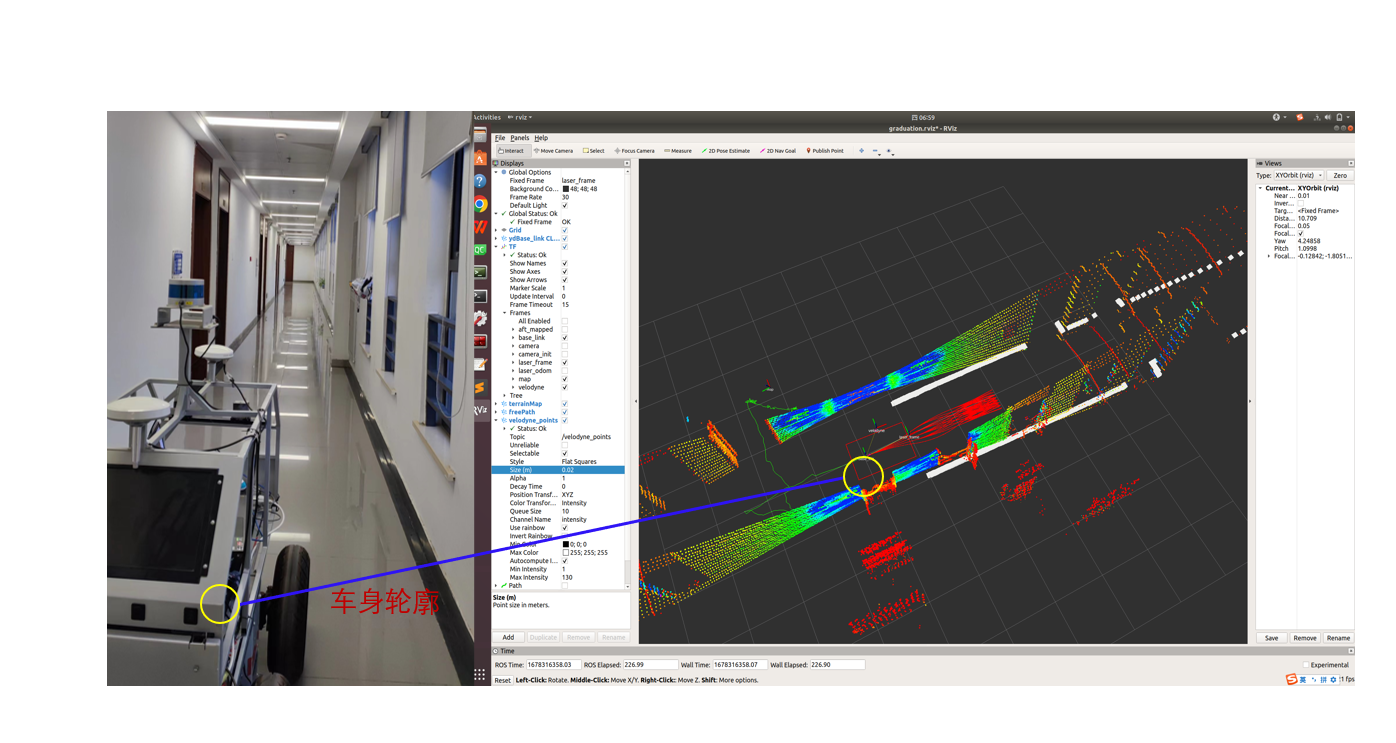
\includegraphics[scale=0.45]{galleyEnv1.png}
    \caption{狭窄环境下的路径组与环境}
\end{figure}
本文在处理实际的路径组和静态障碍物时,对车身进行了一定体积的膨胀,以车体的轮廓为为基准,安全性为第一要求,对车身周围一定范围内的障碍物都保持一定的安全距离。



\subsubsection{最优路径选择}
此刻,底层导航系统接收到一个局部目标点,位于车身的某个位置,如图所示

\begin{figure}[ht]
    \centering
    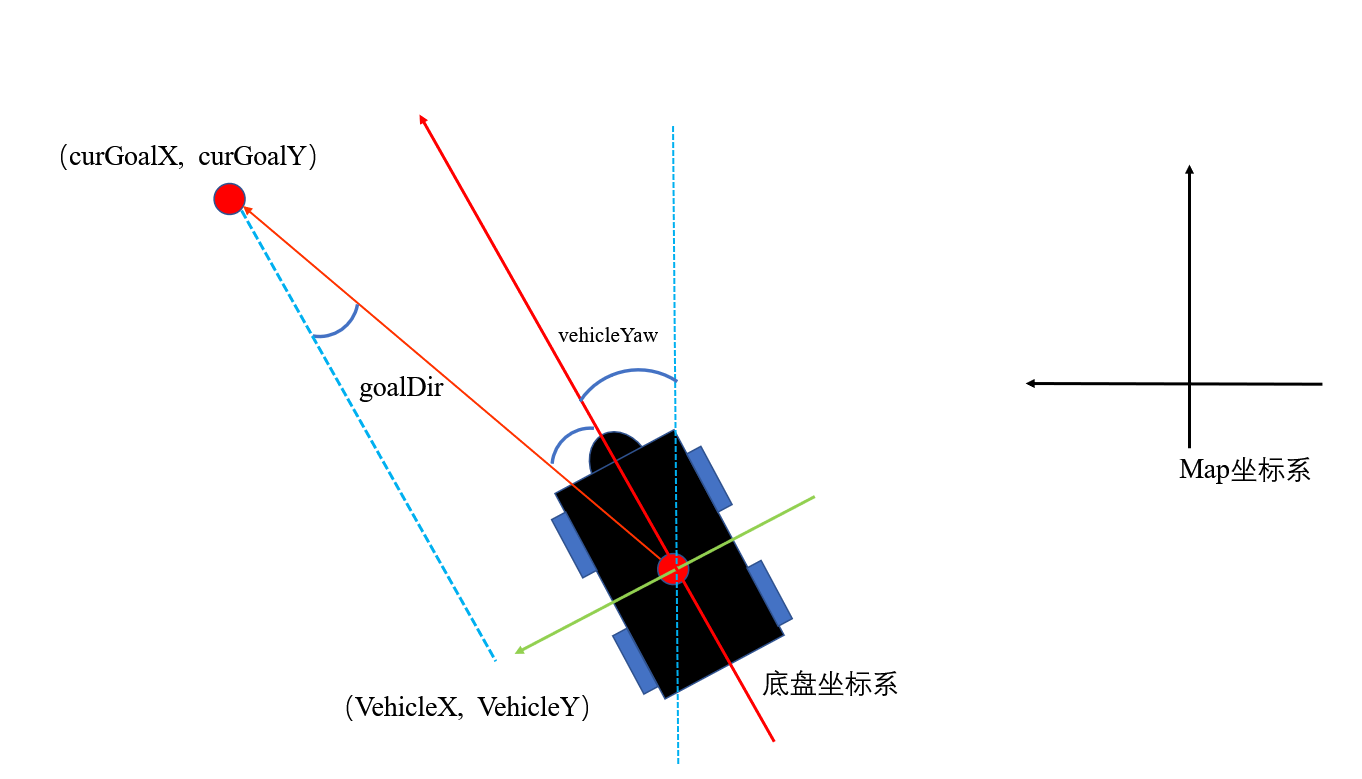
\includegraphics[scale=0.5]{relativeGoal.png}
    \caption{局部目标点与底盘朝向之间的角度拆解}
\end{figure}
图中所示的车身在全局坐标系下的朝向为vehicleYaw,坐标为(VehicleX,  VehicleY)
,局部目标点的全局坐标为(curGoalX, curGoalY),将目标点转换到底盘坐标系下,则目标点在底盘坐标系下的相对坐标为:
\begin{equation}
    \begin{aligned}
        relativeX = ((curGoalX - vehicleX) * cos(vehicleYaw) \\
        + (curGoalY - vehicleY) * sin(vehicleYaw)) \\
        relativeY = (-(curGoalX - vehicleX) * sin(vehicleYaw) \\
        + (curGoalY - vehicleY) * cos(vehicleYaw))
    \end{aligned}
\end{equation}

如图5.6所示为计算某条路径的速度方向的方式,在底盘坐标系下,要转向局部目标点的方向,需要的转向角度为goalDir:
\begin{equation}
    goalDir = atan2(relativeY, relativeX)
\end{equation}

运动元路径组中共9*9*9条路径中第$i$条路径的角度为pathDir,那么第$i$条路径与目标点方向的角度差值为:
\begin{equation}
    angDiff = \left\lvert goalDir - pathDir\right\rvert 
\end{equation}

对运动元路径组进行障碍物点云以及坡度点云按照式(3.16)方式转换到车体坐标系下,并且通过上述的体素网格与路径组的对应关系,剔除所有会影响到移动机器人车身的路径。使用penaltyList[$i$]记录下路径中第$i$条路径上坡度点云的相对高度值,若没有坡度点云存在于第$i$条路径上,penaltyList[$i$] = 0。
据此计算坡度惩罚项,记作penaltyScore[$i$]:
\begin{equation}
    penaltyScore\left[i\right] = 1 - \lambda * penaltyList\left[i\right] 
\end{equation}

$\lambda$为系数,可以人为调节,影响移动机器人局部规划时对坡度点云的厌恶程度。

最后对第$i$条路径的评分为:
\begin{equation}
    score = (1 - \sqrt{\sqrt{0.005*angDiff}})*penaltyScore\left[i\right]
\end{equation}

如图3.9所示对每个group中的所有存在路径(不包含已经因障碍物遮挡剔除的路径)都进行遍历计算,最终得到整个组中所有的角度的评分和。
然后排序所有的group评分,选择评分最高的那个group的路径组中的第一段,也就是三次模拟生成路径的第一段交给运动控制部分进行执行。







\subsection{运动控制}
采用路径跟随法进行运动控制,这也是本文提前生成离线运动元的原因之一。运动控制部分以选择好的路径组运动元为依托,每根运动元路径保存有相应的速度信号。根据上述算法选择了路径组之后,相应的速度:linear 和 angular都是确定的。

\subsection{局部区域的底层导航方法验证实验}
为了正式局部导航方法的鲁棒性与在实地场景使用的可行性,本文将按照局部导航方法构建的底层导航子系统以硬件形式搭建出来后,在校园的室内场景与室外场景下,分别进行了实验。为证实系统在室内室外场景下的功能通用性,在室内场景下,以LeGO-LOAM为底层导航的定位方式,在地下车库环境下进行路径点追踪实验;在室外场景下以RTK作为定位手段,通过预录制的路径点,围绕实验大楼做了一次底层导航的实验。实验的过程图片以及结果展示均来自于实地场景运行过程中的ROS系统封rviz截图,实验展示图中所有白线为发布的路径,蓝色线条为系统运行过程的实际路线
实验结果以及过程中的终端界面以及定位方式的改变导致的tf树等变换关系呈现如下:
\subsubsection{室内基于LeGO-LOAM的局部导航实验}
本文的主要工作在于通用系统的构建,因此对于定位的追求在于定位系统的室内外可切换性,并不过度追求定位模块的精度,且根据目前移动机器人系统的计算核心算力考虑,采用计算资源消耗与定位精度平衡较好的LeGO-LOAM作为室内定位的方法。实验的真实场景与系统的界面如下图所示:

\begin{figure}[ht]
    \centering
    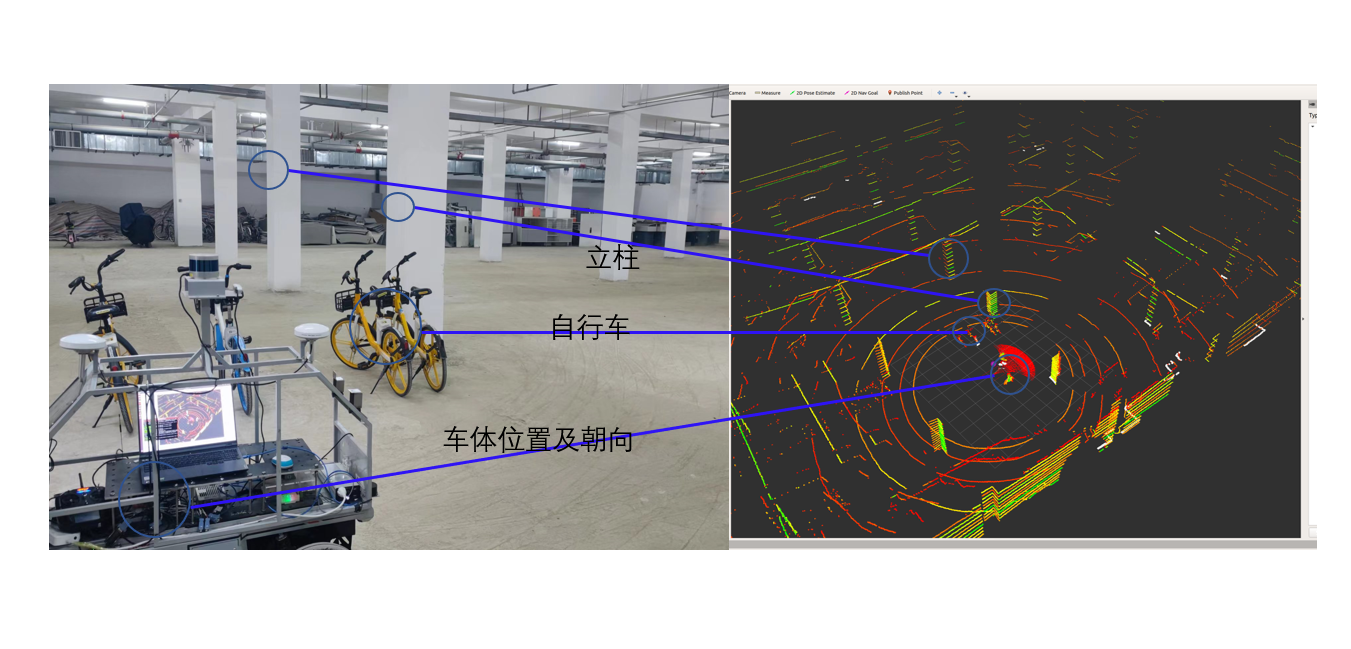
\includegraphics[scale=0.5]{garageScene.png}
    \caption{地下车库场景实物与系统局部点云对比}
  \end{figure}
场景内有多处静态障碍物以及立柱,可以很好地显示出系统在无高层全局规划前提下,对室内目标点的追踪以及通过路径避障方式躲避静态障碍物的性能。

首先给系统发布一系列规则的点,模仿一定条件下对单点的导航能力。

\begin{figure}[ht]
    \centering
    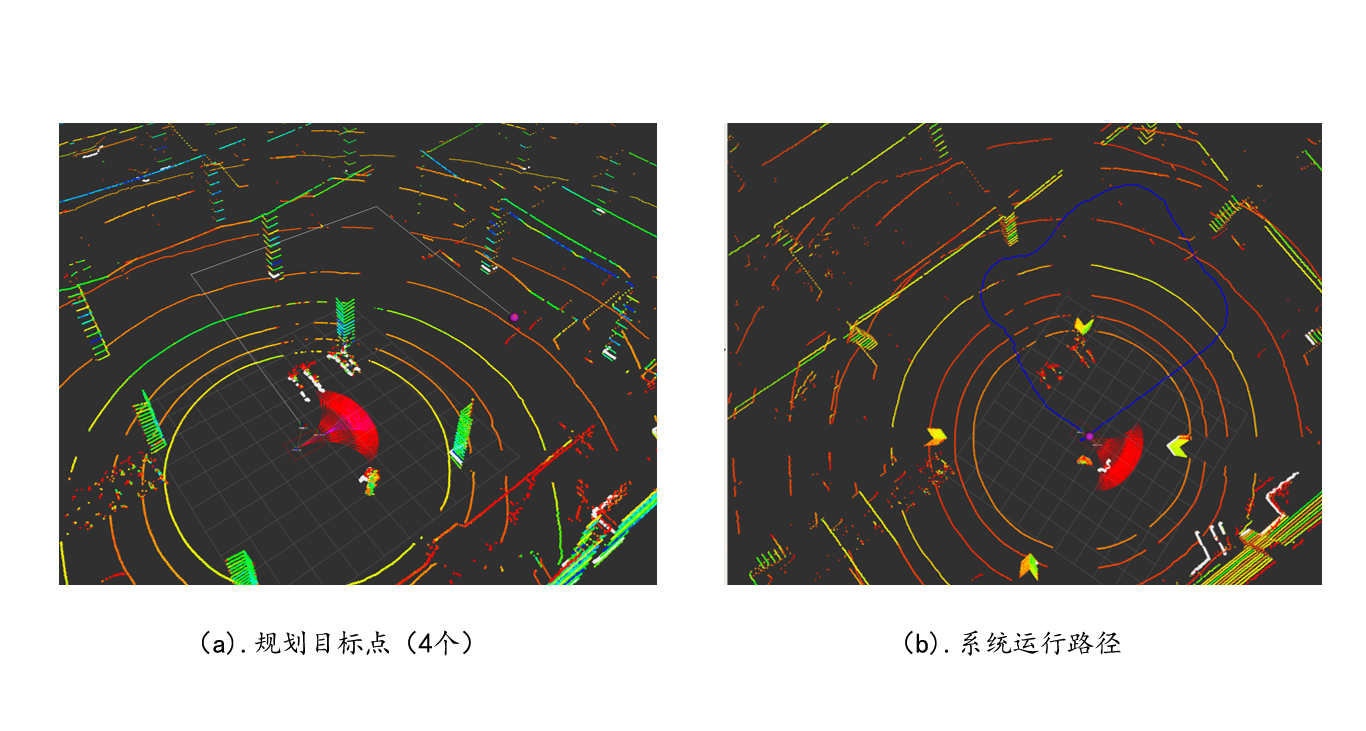
\includegraphics[scale=0.5]{gara_4p.png}
    \caption{系统追踪指定多个目标点运行结果}
  \end{figure}

上图(a)表示在系统运行之初规划的4个目标点的位置,四个目标点连成一个矩形,系统按照矩形运行一周,并最终回到初始位置。(b)中蓝色轨迹为小车运行时记录下的实际位置。可以看出系统可以按照目标点的给定鲁棒地追踪目标点。

然后按照上图目标点让系统二次运行,并在一定位置给于简单动态人体阻碍,运行的结果和对比如下图所示:
\begin{figure}[ht]
    \centering
    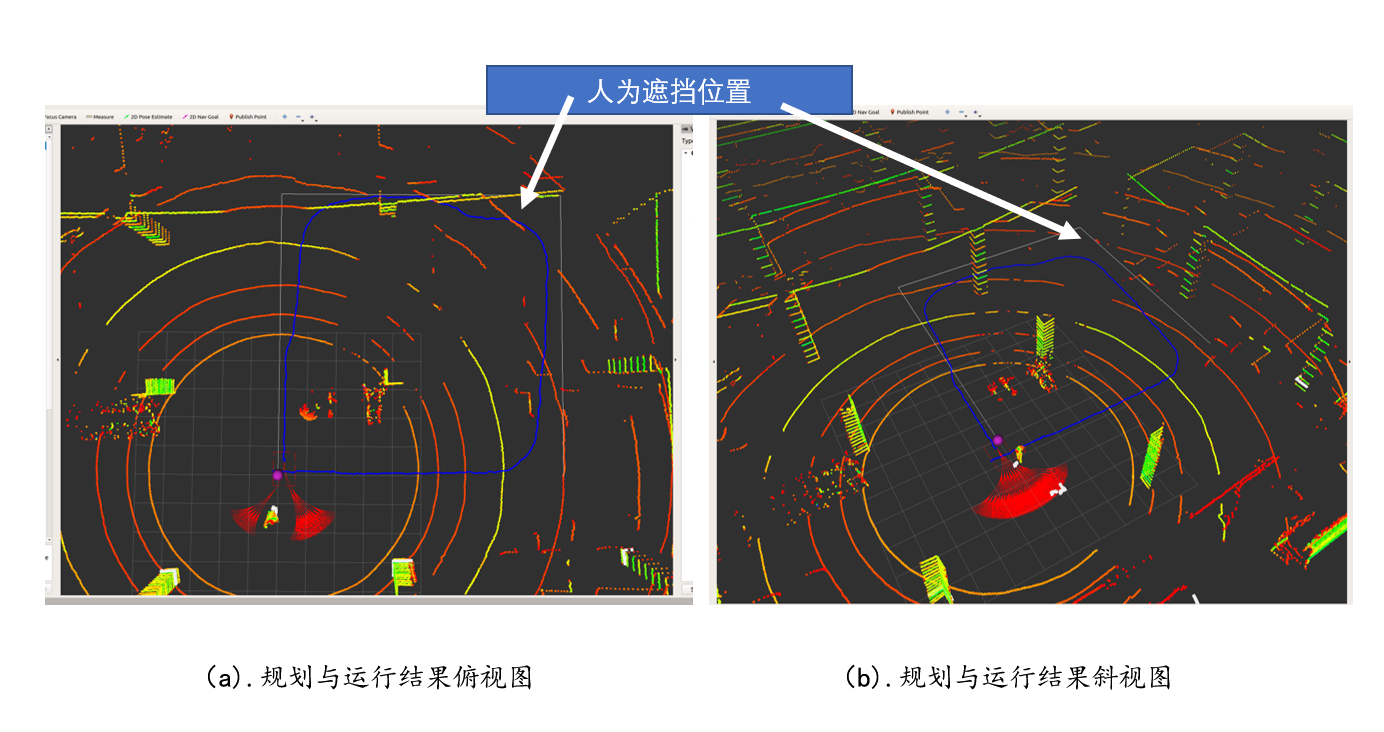
\includegraphics[scale=0.4]{gara_4p_dynam.png}
    \caption{二次运行并施加动态遮挡}
  \end{figure}
如图所示,系统的目标点不变情况下,在第二个目标点出施加简单的动态遮挡,系统可以根据点云的位置作出实时反应,在判定到达目标点后向着下一个目标点做紧急转向,以避免可能发生的碰撞。同时系统二次运行的路线与第一次运行的轨迹有所差异,这是系统设计中并没有刻意去规定转向的优先级往左或者往右,而是给了系统在运行时更多的自主权力,为简单避障留有裕量。

下图将展示系统具体运行时的过程轨迹,展现完整的追踪目标点的过程,图中的紫色点是当前时刻系统所需要移动指向的目标点,在抵达某一个目标点后,才会向着下一个目标点进发,其详细过程和终端界面的输出如下图所示:

\begin{figure}[ht]
    \centering
    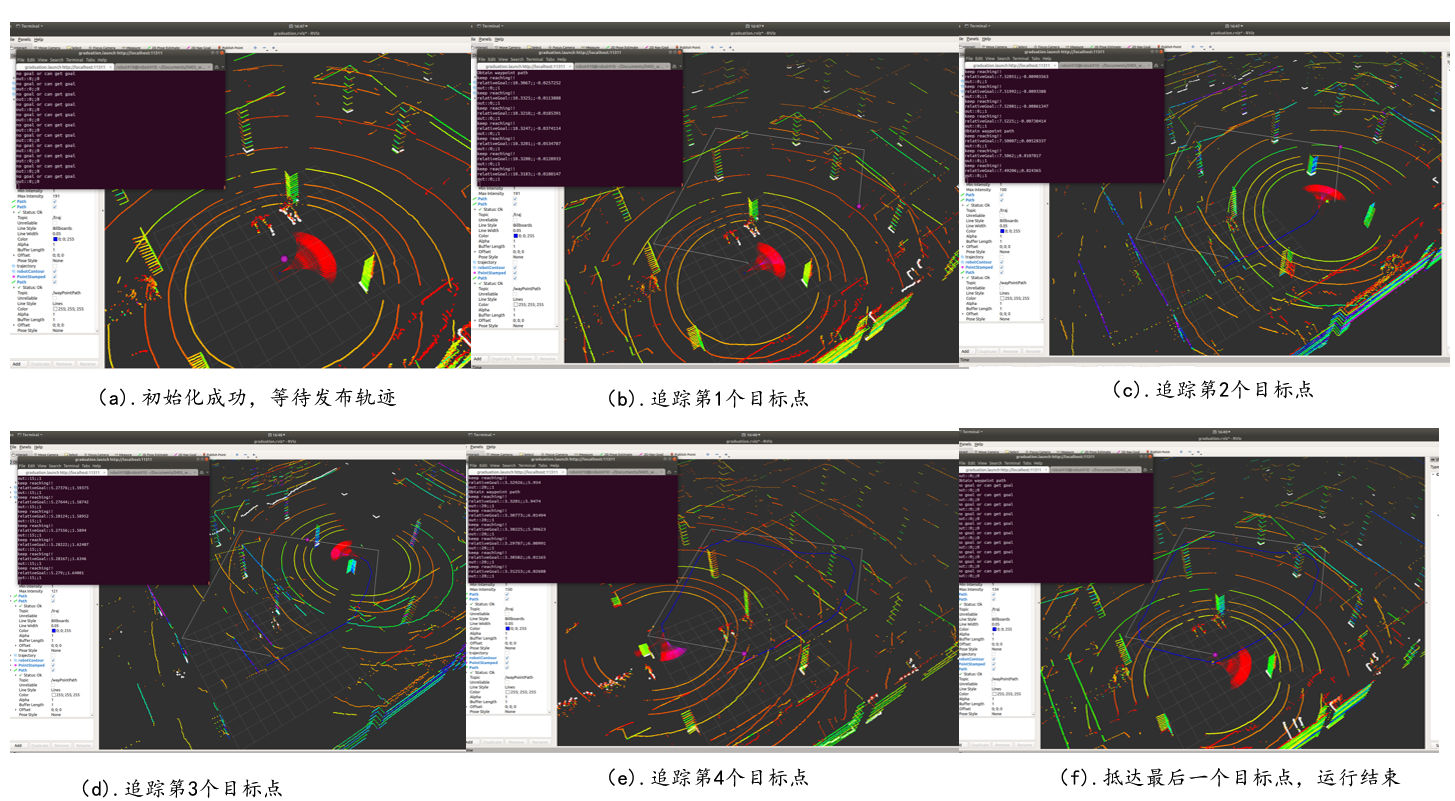
\includegraphics[scale=0.4]{gara_follow.png}
    \caption{对目标点的完整追踪过程以及终端输出}
  \end{figure}
如上图,在局部追踪线程就绪后,等待目标点发布后,会沿着一系列目标点行进,最后回到原定位置(也可以将终点目标定在非原始位置)。运行的过程图完整如上所见。

接下来为了展示系统在不同场景下的应用鲁棒性,在两个场景下,进行了路点录制以及跟踪展示,录制路点并二次发布的过程是为了模拟在实际应用中高层导航下发的场景全局路径过程,同时,由于路点录制可以随心所欲,故可在录制过程中增加大量复杂性条件,可更好地测试底层导航的性能。

轨迹一:录制距离3m, 目标点的到达容忍度为1.5m,结果展示如图:

\begin{figure}[ht]
    \centering
    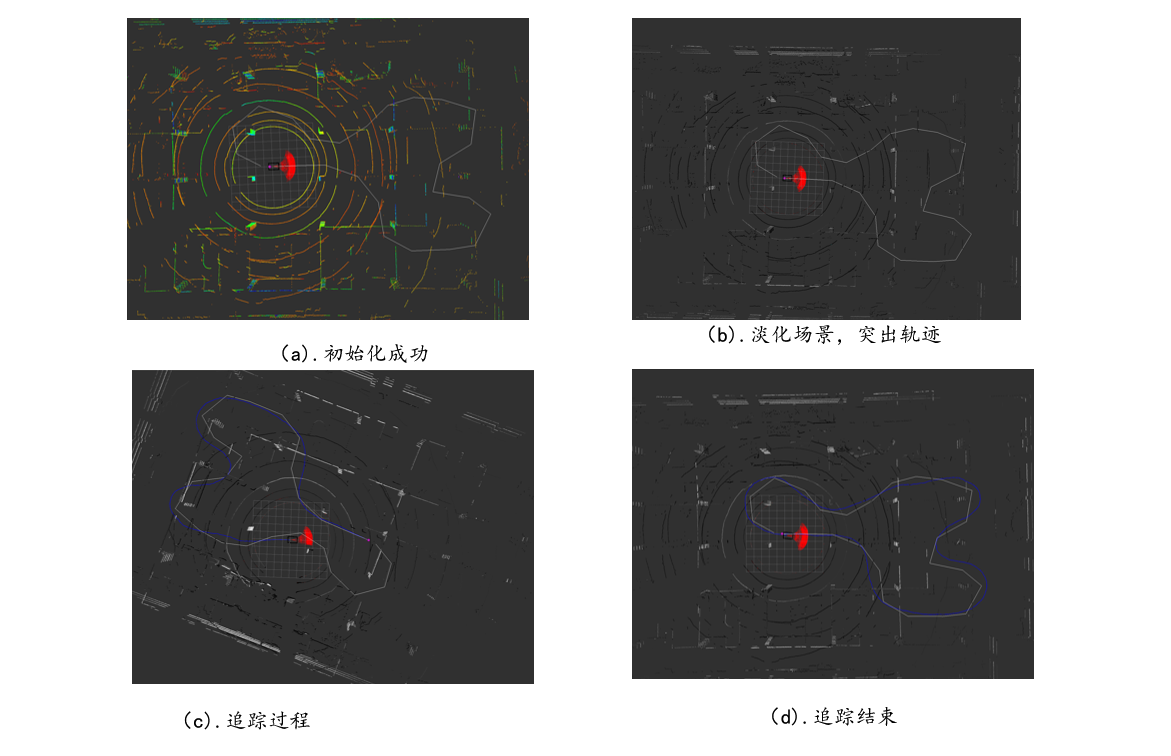
\includegraphics[scale=0.5]{gara_pathpoints.png}
    \caption{室内对路点的追踪过程}
  \end{figure}

轨迹的对比结果如图所示:

\begin{figure}[ht]
    \centering
    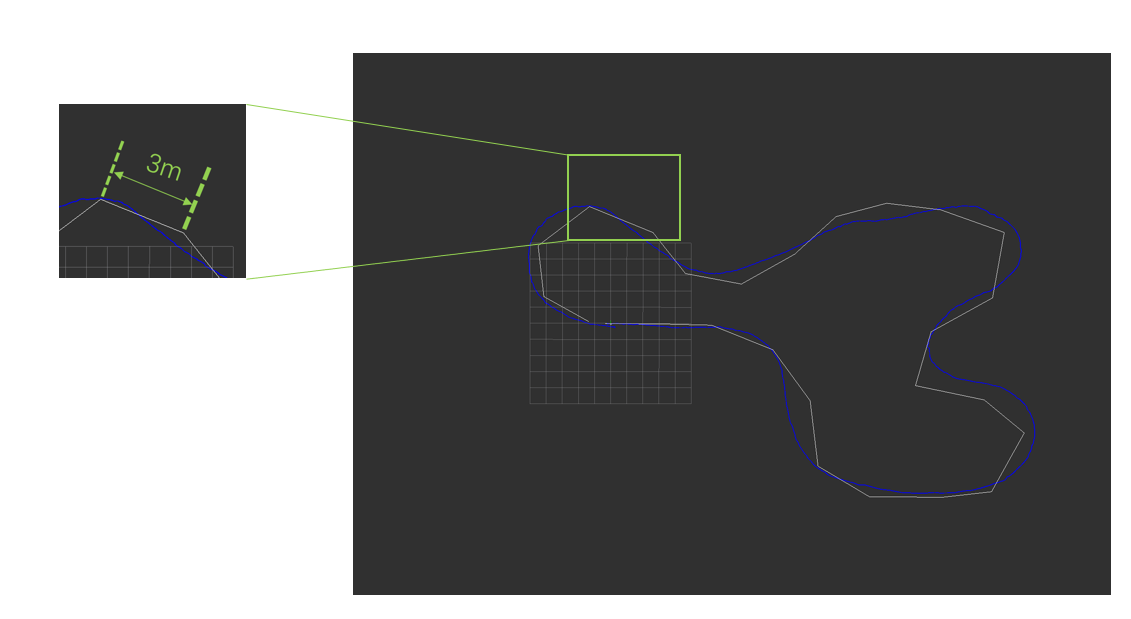
\includegraphics[scale=0.4]{gara_cmp2.png}
    \caption{轨迹对比1}
  \end{figure}

此轨迹一录制共录制路点27个,全长约为81m。
录制路点的时候,设置路点之间最低距离为3m,即白线折点之间的连线长度为3m,车体到达目标点范围内1.5视为到达当前目标点,系统开始下发下一个目标点并追踪。

轨迹二:录制距离1m, 目标点的到达容忍度为1m,图形为简单凸边形,结果展示如图:
\begin{figure}[ht]
    \centering
    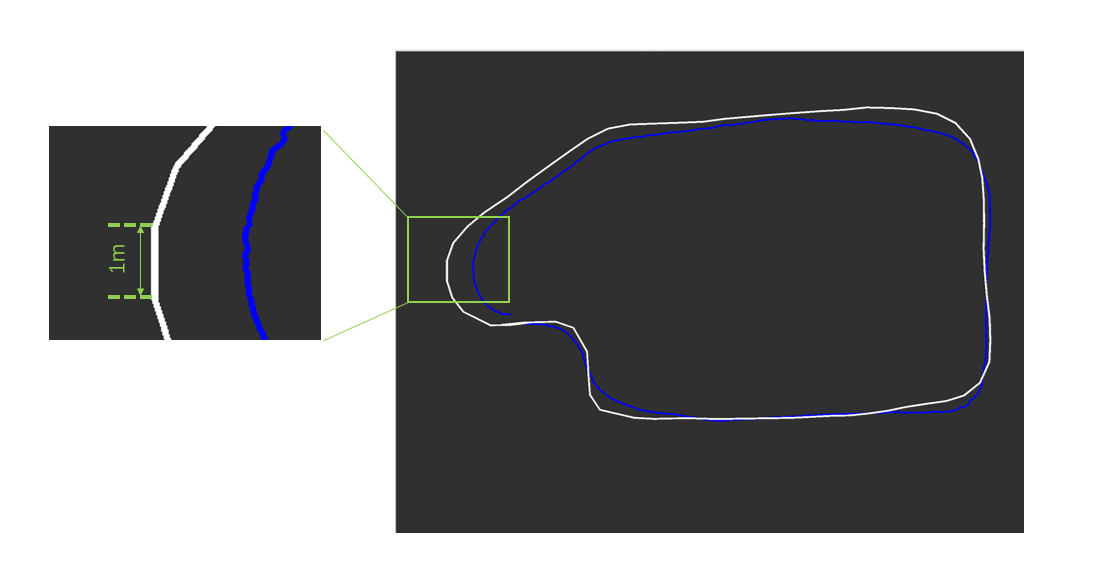
\includegraphics[scale=0.4]{gara_cmp3.png}
    \caption{轨迹对比2}
  \end{figure}
此轨迹一录制共录制路点69个,全长约为69m。
录制路点的时候,设置路点之间最低距离为1m,即白线折点之间的连线长度为3m,车体到达目标点范围内1m视为到达当前目标点.

轨迹三:录制距离1m, 目标点的到达容忍度为1m,图形为复杂的轨迹曲线,结果展示如图:

\begin{figure}[ht]
    \centering
    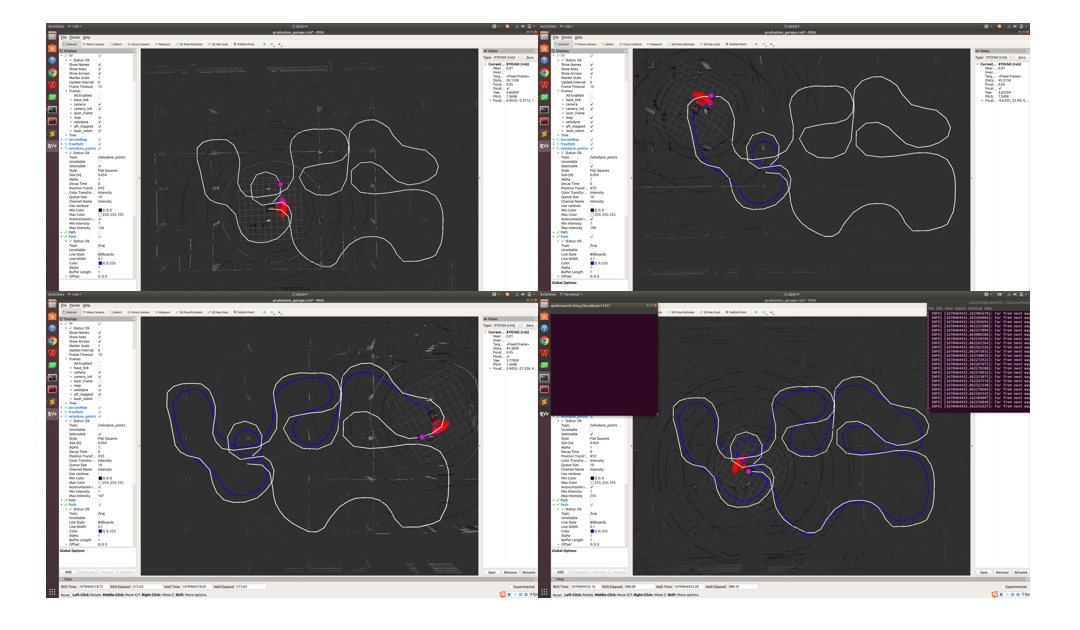
\includegraphics[scale=0.4]{gara_process.png}
    \caption{运行过程}
  \end{figure}

\begin{figure}[ht]
    \centering
    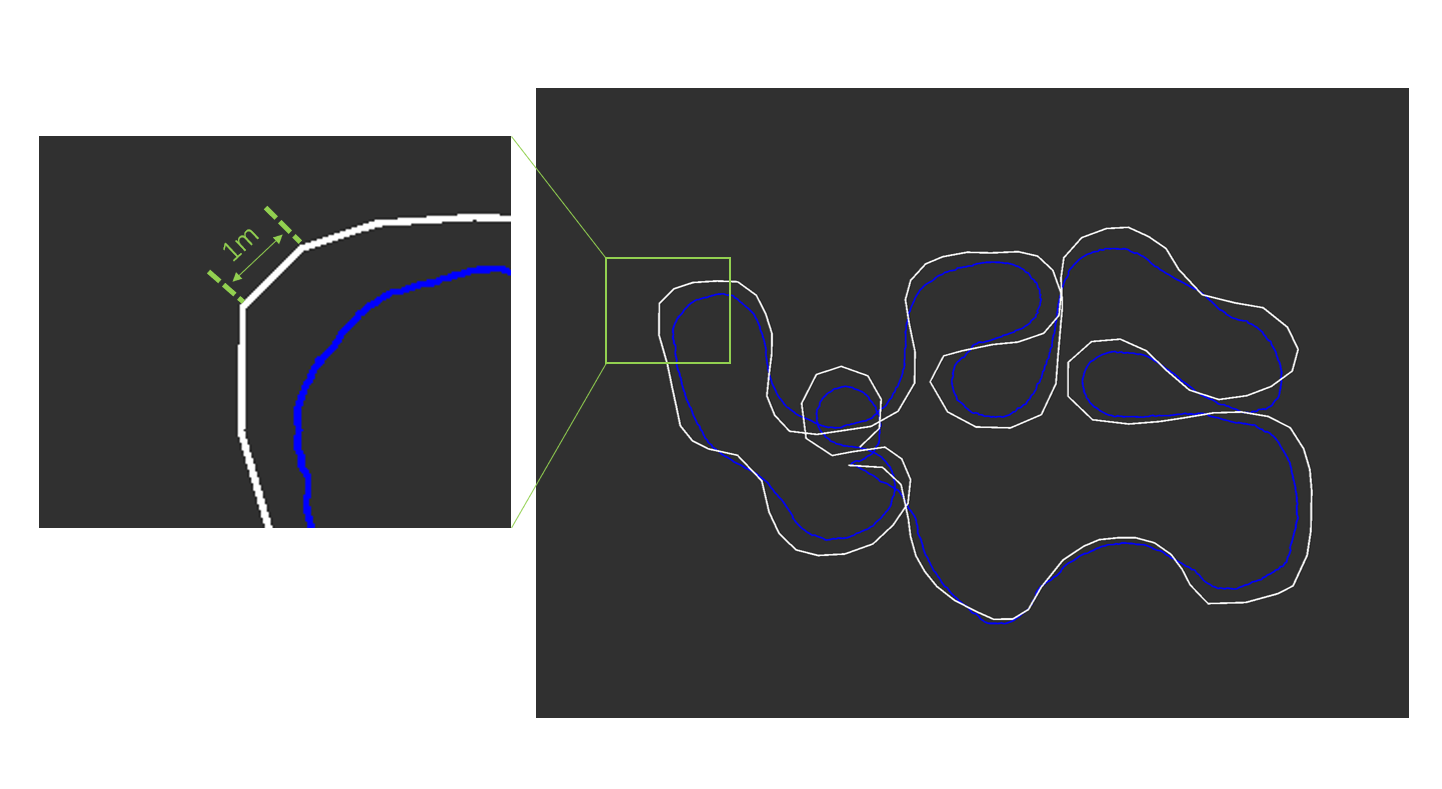
\includegraphics[scale=0.4]{gara_cmp4.png}
    \caption{轨迹对比}
  \end{figure}
此轨迹一录制共录制路点140个,全长约为140m。

从以上几段轨迹的实验可以证明,我们搭建的移动机器人在室内可以使用SLAM方法对环境实时定位并跟踪相应的全局轨迹,随着算法的路点采集距离以及目标点的到达容忍度设置减小,轨迹跟踪的精度也愈高,但是受限于实验室阿克曼平台本身的体积和约束,目前的效果依然有待提升。若改换成体积较小的移动机器人,算法的精准度可以再次提高。


\subsubsection{室外基于路点的大场景实验}
上述实验的目的更多是证明相应室内导航算法的室内可用性,在室外使用RTK进行定位,并对在学校内的大型区域内进行了路点的录制与导航跟踪实验。本次实验的路点录制距离均为3m,到达目标的容忍度为2m。录制了两端轨迹,分别展示了园区运行的范围以及园区内运行过程中的多转弯等轨迹实验。室外的RTK选定的坐标原点以及车身在园区内对应的坐标系tf关系如图所示:

\begin{figure}[ht]
    \centering
    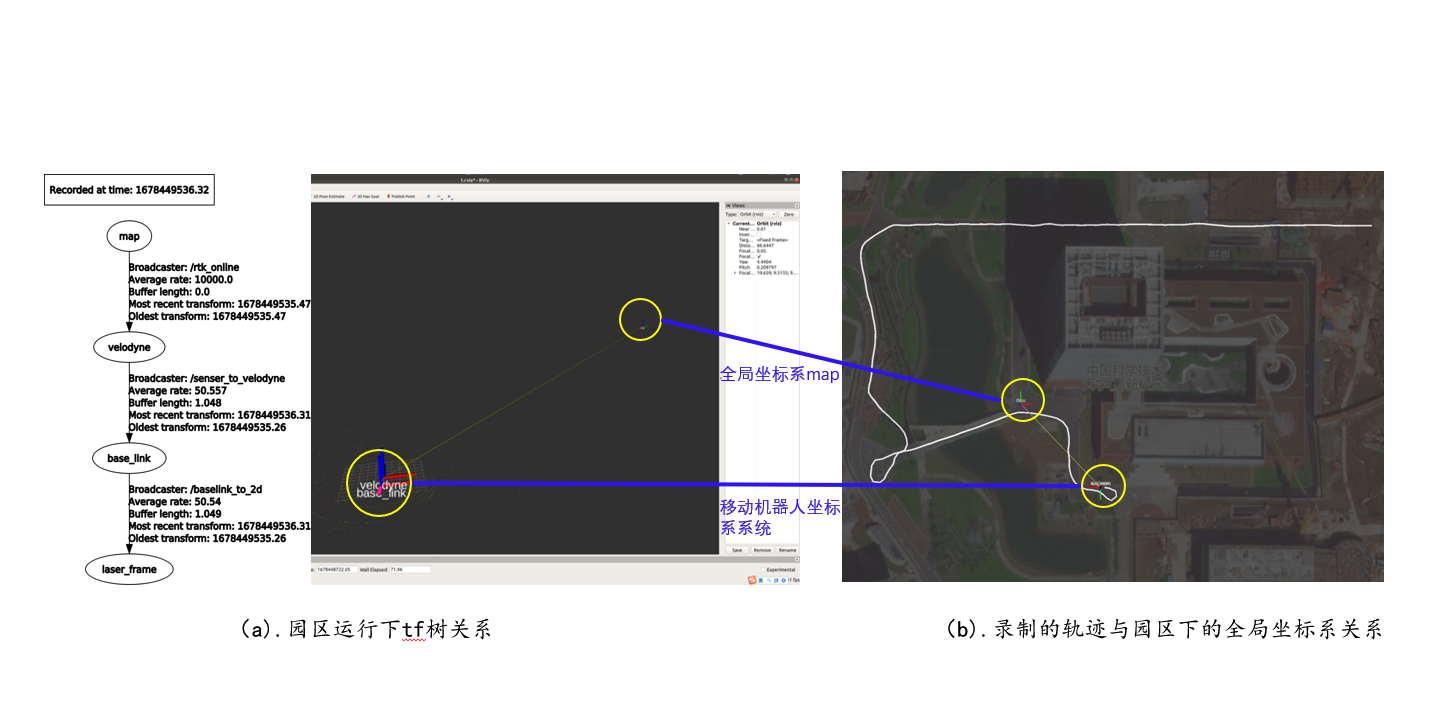
\includegraphics[scale=0.45]{campusAxis.png}
    \caption{园区场景下的坐标系关系与实景对照1}
  \end{figure}



轨迹一: 目标点的到达容忍度为2m,其过程展示图如下:

\begin{figure}[ht]
    \centering
    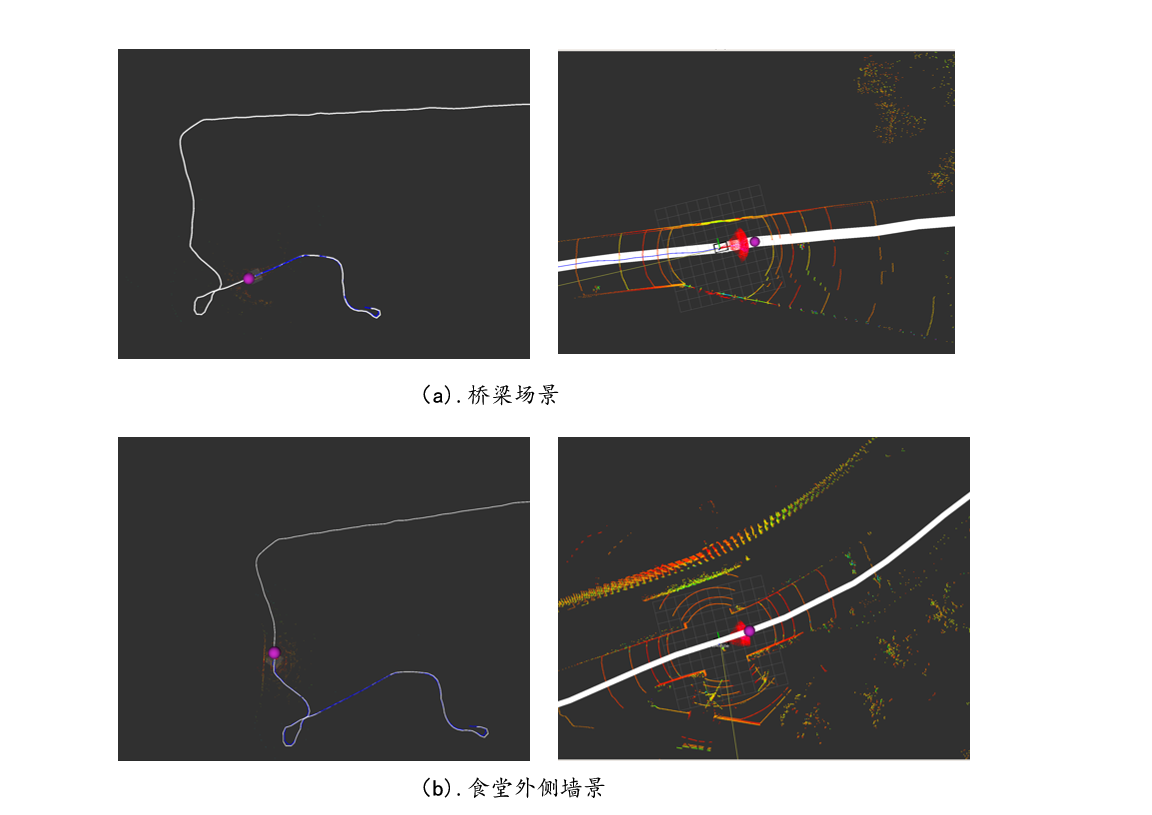
\includegraphics[scale=0.5]{campus_bridge.png}
    \caption{园区场景下的常轨迹追踪过程及其局部放大图}
  \end{figure}

轨迹的对比结果如图所示:

\begin{figure}[ht]
    \centering
    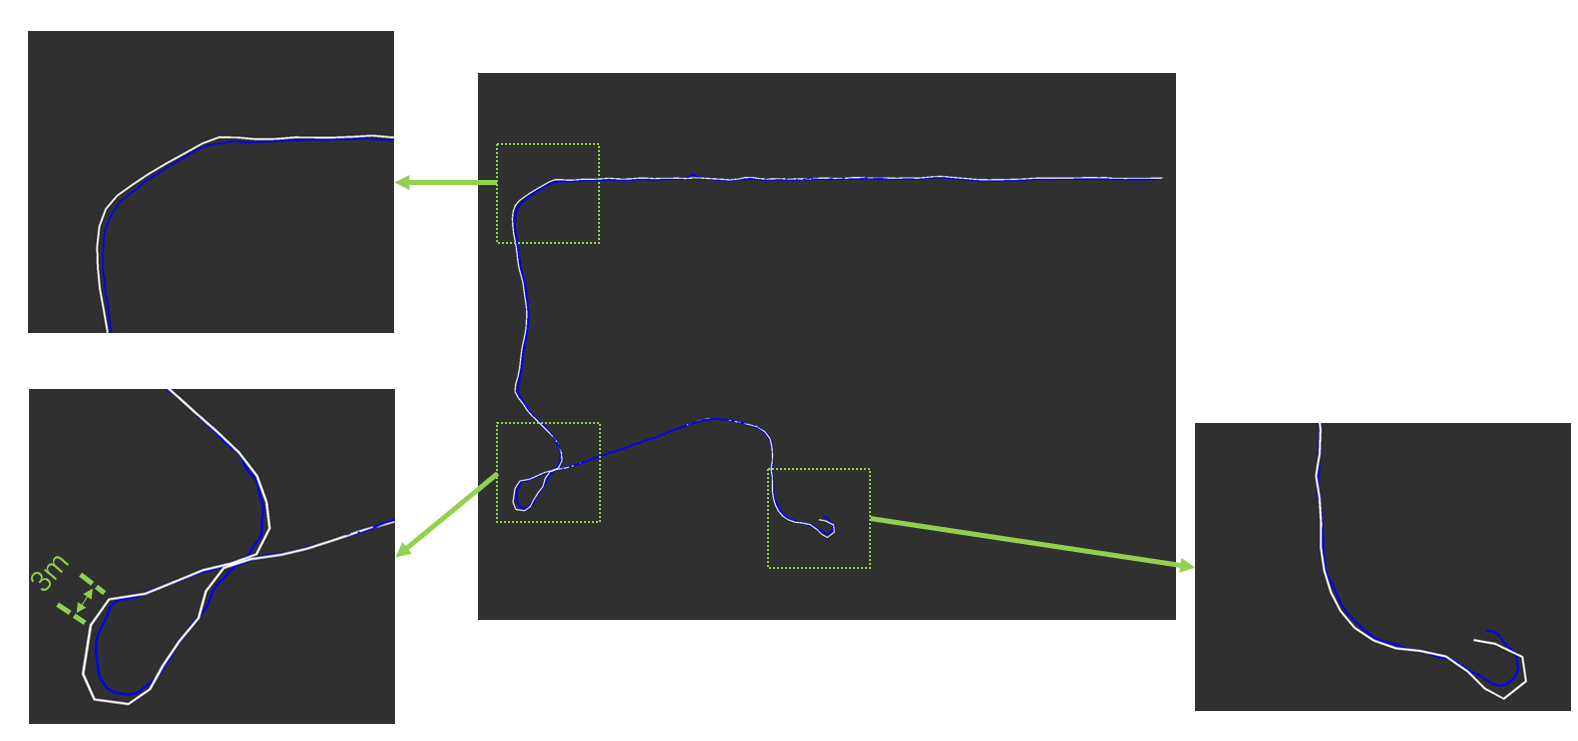
\includegraphics[scale=0.4]{campus_cmp1.png}
    \caption{园区轨迹1对比及其局部放大效果图}
  \end{figure}

此轨迹一录制共录制路点420个,全长约为1200m。


轨迹二: 目标点的到达容忍度仍为2m,但选择的是园区内弯绕路线,测试系统在园区内的方向选择能力,实景图如下所示:

\begin{figure}[ht]
    \centering
    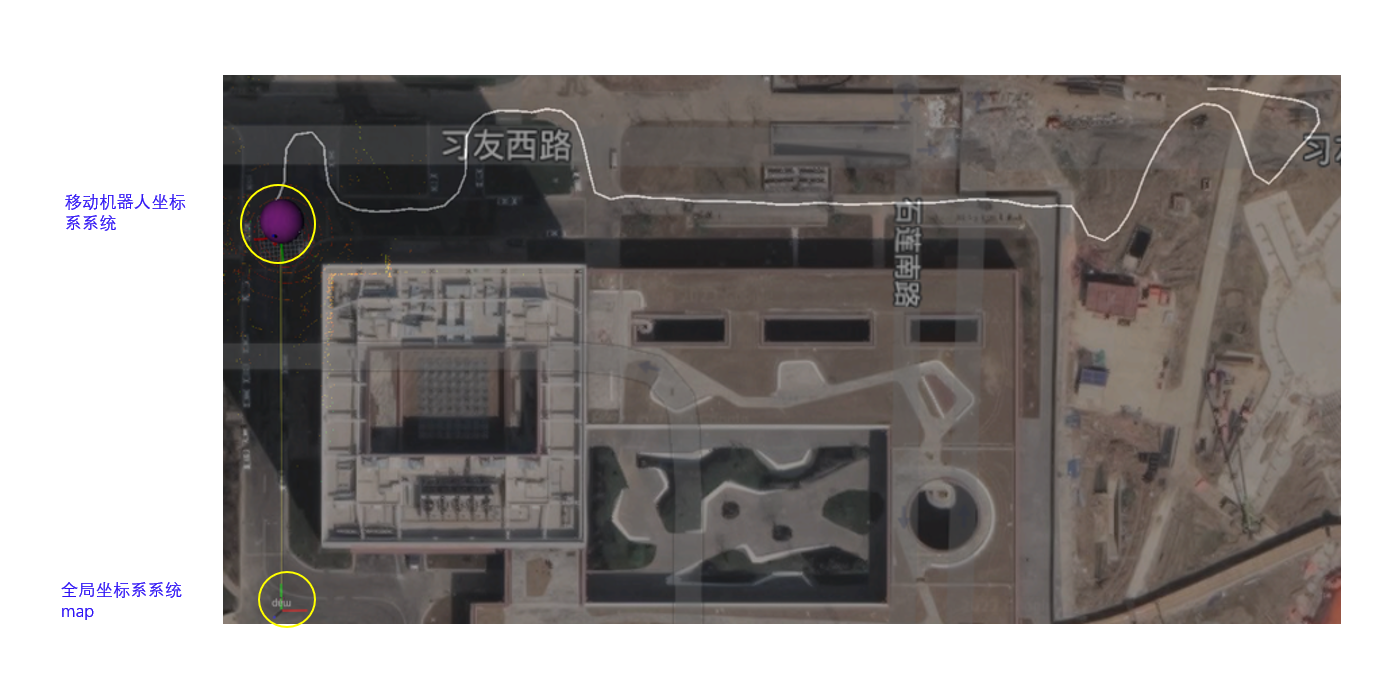
\includegraphics[scale=0.45]{campusAxis2.png}
    \caption{园区场景下的坐标系关系与实景对照2}
  \end{figure}

轨迹的对比结果如图所示:

\begin{figure}[ht]
    \centering
    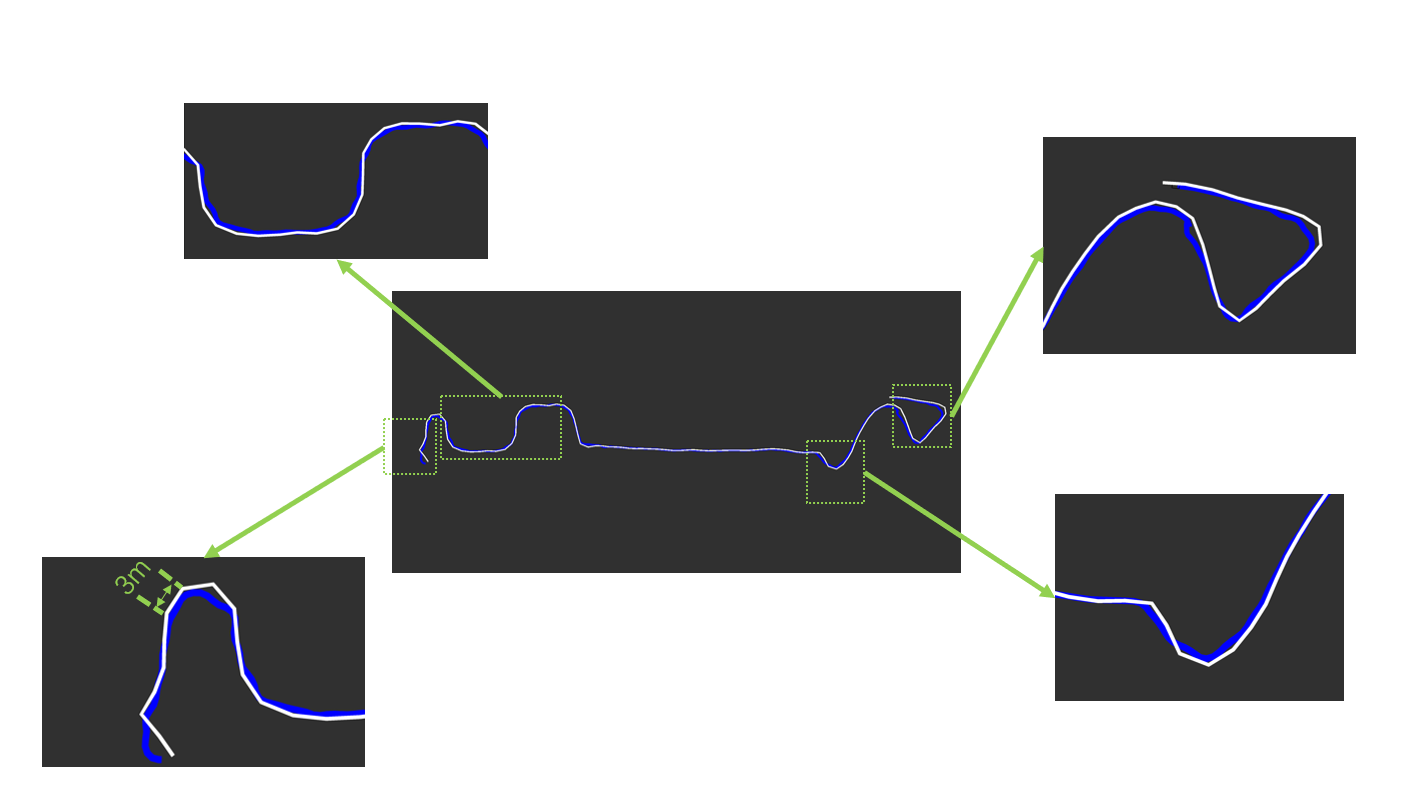
\includegraphics[scale=0.4]{campus_cmp2.png}
    \caption{园区轨迹2对比及其局部放大效果图}
  \end{figure}
此轨迹一录制共录制路点130个,全长约为400m。

结论:经实验验证发现,在室外场景下,随着RTK的使用,其定位精度比室内场景下的LeGO-LOAM高,故导航系统的轨迹跟随准确性也随之升高。据此两个实验,验证底层局部导航的功能,并且验证了系统在室内外切换使用的可行性。



















